% ============================================================================
% BTech Final Report
% Project: A Multimodal Framework for Agricultural Drought Monitoring and Prediction
% Figures: figures/*.png (generated by final_report_materials/make_diagrams.py with NO_TITLE=1)
% Logo:    figures/logo.jpeg
% UAV section (Sec. 7) is provisional, taken from the mid-review; marked "% UAV-TODO".
% ============================================================================

\documentclass[11pt,a4paper,oneside]{article}

% ============================== PAGE LAYOUT ==================================
\usepackage[left=0.62in,right=0.62in,top=0.5in,bottom=0.5in]{geometry}
\usepackage[utf8]{inputenc}
\usepackage[T1]{fontenc}
\usepackage{lmodern}
\usepackage{amsmath}
\usepackage{amssymb}
\usepackage{graphicx}
\graphicspath{{./}{figures/}{figures/figures/}} % finds figures in figures/ or figures/figures/
\usepackage{booktabs}
\usepackage{array}
\usepackage{tabularx}
\usepackage{multirow}
\usepackage{enumitem}
\usepackage[dvipsnames]{xcolor}
\usepackage[colorlinks=true,linkcolor=NavyBlue,citecolor=ForestGreen,urlcolor=RubineRed]{hyperref}
\usepackage{titlesec}
\usepackage{tikz}
\usetikzlibrary{shapes.geometric,shapes.symbols,arrows.meta,positioning,backgrounds,fit}
\usepackage{float}
\usepackage{caption}
\captionsetup{font=small,labelfont=bf}

% ============================ COMPACT ACADEMIC STYLE ==========================
\setlength{\parindent}{0pt}
\setlength{\parskip}{3pt}

\titleformat{\section}{\fontsize{13pt}{16pt}\selectfont\bfseries}{\thesection.}{5pt}{}
\titleformat{\subsection}{\fontsize{11.5pt}{14.5pt}\selectfont\bfseries}{\thesubsection}{5pt}{}
\titleformat{\subsubsection}{\fontsize{10.5pt}{13pt}\selectfont\bfseries}{\thesubsubsection}{5pt}{}
\titlespacing*{\section}{0pt}{6pt}{3pt}
\titlespacing*{\subsection}{0pt}{4pt}{2pt}
\titlespacing*{\subsubsection}{0pt}{3pt}{1pt}

\setlist{nosep,leftmargin=1.3em,itemsep=2pt,topsep=3pt}
\renewcommand{\arraystretch}{1.0}
\tolerance=1500
\emergencystretch=2em
\hyphenpenalty=300

\newcolumntype{Y}{>{\raggedright\arraybackslash}X}
\newcommand{\mf}{macro-F1}

% ============================================================================
\begin{document}

% ============================== FRONT PAGE ==================================
\begin{titlepage}
\thispagestyle{empty}
\begin{center}
\vspace*{2.8cm}

{\LARGE\bfseries
A Multimodal Framework for Agricultural Drought Monitoring and Prediction using Weather Time Series, Satellite Imagery, and UAV Semantic Segmentation\par}

\vspace{1.9cm}
{\large\bfseries B.Tech in Computer Science and Engineering\par}
\vspace{0.45cm}
{\normalsize by\par}
\vspace{0.25cm}
{\large\bfseries
\renewcommand{\arraystretch}{1.2}
\begin{tabular}{ll}
G. ARYAN RAJESH & (123CS0020) \\
M. ROVAN & (123CS0036) \\
M. HARSHA VARDHAN & (123CS0044) \\
\end{tabular}\par}

\vspace{0.55cm}
{\normalsize Under the Guidance of\par}
\vspace{0.15cm}
{\normalsize\bfseries Dr. M. NARESH BABU\par}
{\normalsize Associate Professor\par Dept. of CSE\par}

\vspace{1.25cm}

\includegraphics[width=3.0cm]{figures/logo.jpeg}
\vspace{1.25cm}

{\small\bfseries DEPARTMENT OF COMPUTER SCIENCE AND ENGINEERING\par}
{\small IIITDM KURNOOL\par}
\vspace{0.35cm}
{\small November 2026\par}
\end{center}
\end{titlepage}

\clearpage
\setcounter{page}{2}

% ============================== ABSTRACT ====================================
\section*{Abstract}
Agricultural drought in semi-arid Rayalaseema (Andhra Pradesh) and neighbouring Tumakuru (Karnataka) is officially declared only late in the season. This project builds a three-stage early-warning chain: a \textbf{weather module} forecasts meteorological drought (SPEI-30 class) 7, 15 and 30 days ahead; a \textbf{satellite module} confirms whether crops on randomly sampled Sentinel-2 fields actually became stressed; and a \textbf{UAV module} quantifies the damaged area on flagged fields. Because rabi (winter) crops depend on stored soil water and irrigation rather than current rain, a separate \textbf{rabi module} forecasts crop greenness 15 days ahead.
All modules are evaluated on held-out years, with calibrations frozen on training periods, purged chronological splits, automated leakage tests, strong simple baselines and rules fixed before evaluation; government drought orders are used only as an independent comparison.
The hybrid physics + machine-learning weather model reaches \mf{} 0.819 / 0.651 at 7 / 15 days (persistence 0.662 / 0.515; 85.6\,\% balanced accuracy at 7 days). Rainfed crop greenness follows 30-day SPEI with a 10-day lag ($\rho = 0.45$ on unseen years). In an operational replay with realistic data delays, the weather-to-satellite chain confirmed all 9 severe kharif drought site-seasons declared in 2023--2026 (5 before the government order) with 1 false alarm in 11 undeclared site-seasons. For rabi, an XGBoost forecast of NDVI 15 days ahead had about 18\,\% lower mean absolute error than the best simple baseline in three held-out seasons (historical evaluation).

\vspace{4pt}
\textbf{Keywords:} agricultural drought, SPEI, Sentinel-2, XGBoost, early warning, rabi, UAV segmentation.

% ============================================================================
\section{Introduction}

Agricultural drought is a recurring threat to rainfed farming in India's semi-arid Rayalaseema region, where groundnut, cotton, maize and pulses depend on the south-west monsoon (kharif, June--November) and, in winter (rabi, October--April), on stored soil moisture and limited irrigation. Drought is declared by the state government following the \textit{Manual for Drought Management}~\cite{manual2016}, but orders arrive late in the season (kharif orders in October--November, rabi orders in mid/late March), and a national comparison of detected and declared droughts found detection weakest in Andhra Pradesh and Karnataka~\cite{bhardwaj2021}. In 2023--2026 the Government of Andhra Pradesh declared drought in several of our study mandals in both seasons.

Existing approaches usually work in isolation: weather-index models forecast meteorological drought without checking crops; satellite studies monitor vegetation after the fact, often at district scale; and UAV studies map damage on individual fields but cannot cover a region. This project links the three in a cascade (Fig.~\ref{fig:system}): \emph{the weather alarm says where to look, the satellite says which fields were actually hit, and the drone measures the damaged area}.

\textbf{Contributions.}
\begin{enumerate}
\item A leakage-controlled \textbf{weather module} (AgERA5, 1979--2026, 6 independent cells) with an SPEI calibration frozen on 1979--2011, a physical water-balance ensemble baseline and a physics + ML hybrid model.
\item A \textbf{satellite module} that maps farmland automatically, samples 240 random fields, labels crop condition with the Standardized Vegetation Index (SVI), measures the weather-to-crop lag and replays the system live against four seasons of government orders.
\item A \textbf{rabi module} with rules registered before training: 1,350 random cropland points, explicit missing-data rules and a chronologically tested 15-day NDVI forecast.
\item A \textbf{UAV module} for 7-class semantic segmentation and metric damage area (in progress).
\end{enumerate}

% ============================================================================
\section{Literature Review}

\begin{table}[H]
\centering
\caption{Literature survey: meteorological drought indices and forecasting.}
\label{tab:lit_weather}
\scriptsize
\renewcommand{\arraystretch}{1.05}
\begin{tabularx}{\textwidth}{@{}p{3.1cm}|c|p{2.2cm}|X|X@{}}
\hline
\textbf{Paper} & \textbf{Year} & \textbf{Author} & \textbf{Contribution} & \textbf{Limitation / gap addressed here} \\
\hline
A multiscalar drought index sensitive to global warming: the SPEI~\cite{vicente2010} & 2010 & Vicente-Serrano et al. & Introduced SPEI: climatic water balance ($P-\mathrm{PET}$) fitted with a log-logistic distribution at multiple time scales. & Usually standardised on the full record; we calibrate on 1979--2011 only and freeze the parameters so test years cannot leak into labels. \\
\hline
Long-term SPI drought forecasting in the Awash River Basin using wavelet neural network and wavelet SVR~\cite{belayneh2014} & 2014 & Belayneh et al. & Wavelet-coupled ANN and SVR forecasts of SPI. & Compared only against other ML models; we add persistence, Markov, climatology and a physical water-balance baseline. \\
\hline
An improved SPEI drought forecasting approach using the LSTM neural network~\cite{dikshit2021} & 2021 & Dikshit et al. & LSTM forecasting of monthly SPEI with lower error than stochastic models. & Monthly scale; no strict leakage control or operational delay. We test LSTM and Transformer daily, but tree models with physics inputs perform best. \\
\hline
A review of machine learning methods for drought hazard monitoring and forecasting~\cite{prodhan2022} & 2022 & Prodhan et al. & Review of ML drought forecasting: trends, challenges and future directions. & Highlights validation weaknesses; motivates our frozen calibration, purged splits and confidence intervals. \\
\hline
Long-term drought prediction using deep neural networks based on geospatial weather data~\cite{marusov2024} & 2024 & Marusov et al. & Deep networks predicting drought (PDSI) from gridded weather. & We reproduce their protocol style as a comparison: weather inputs raise 15-day ROC-AUC from 0.81 to 0.89. \\
\hline
\end{tabularx}
\end{table}

\begin{table}[H]
\centering
\caption{Literature survey: satellite monitoring of agricultural drought and the rabi season.}
\label{tab:lit_sat}
\scriptsize
\renewcommand{\arraystretch}{1.05}
\begin{tabularx}{\textwidth}{@{}p{3.1cm}|c|p{2.2cm}|X|X@{}}
\hline
\textbf{Paper} & \textbf{Year} & \textbf{Author} & \textbf{Contribution} & \textbf{Limitation / gap addressed here} \\
\hline
Application of vegetation index and brightness temperature for drought detection~\cite{kogan1995} & 1995 & Kogan & Vegetation Condition Index (VCI): NDVI scaled between historical minimum and maximum. & Needs a long record; with 4--5 reference years about 20\,\% of dates get VCI $\approx 0$ by chance, so we label with SVI. \\
\hline
Drought monitoring with NDVI-based Standardized Vegetation Index~\cite{peters2002} & 2002 & Peters et al. & SVI: z-score of NDVI for a given date. & We compute it per field and day of year with the scored year removed from the normal. \\
\hline
Monitoring agricultural drought for arid and humid regions using multi-sensor remote sensing data~\cite{rhee2010} & 2010 & Rhee et al. & Scaled Drought Condition Index from MODIS LST, NDVI and TRMM rain. & Coarse (MODIS); we link weather and vegetation in time at 10\,m and measure the lag. \\
\hline
Drought assessment and monitoring through blending of multi-sensor indices using machine learning~\cite{park2016} & 2016 & Park et al. & RF, boosted trees and Cubist on 16 MODIS/TRMM drought factors; RF best. & Coarse resolution, index-to-index validation; we validate against government orders and UAV fields. \\
\hline
Drought detection and declaration in India~\cite{bhardwaj2021} & 2021 & Bhardwaj \& Mishra & Compared detected and declared droughts for all districts 2000--2017; lowest detection in AP and Karnataka. & District scale; our study area is the region they flag as hardest, analysed at mandal level. \\
\hline
Integrating EDI and remote sensing derived parameters for agricultural drought assessment and prediction in Bundelkhand~\cite{padhee2014} & 2014 & Padhee et al. & Rabi-season (Oct--Apr) drought; NDVI anomaly predicted from soil-moisture anomaly with a 16-day lag. & MODIS 250\,m, linear model; we forecast 10\,m NDVI with XGBoost on held-out seasons. \\
\hline
Prediction of vegetation anomalies to improve food security and water management in India~\cite{asoka2015} & 2015 & Asoka \& Mishra & Forecast NDVI anomalies 1--3 months ahead over India. & Regional scale; ours is field-point scale with eligibility rules for cloud gaps. \\
\hline
Evaluating Sentinel-2 for monitoring drought-induced crop failure in winter cereals~\cite{descals2025} & 2025 & Descals et al. & Early decline of Sentinel-2 indices in drought-hit winter cereals ($R^2 = 0.66$). & Temperate cereals with field survey; our decline warnings cannot yet separate drought from harvest. \\
\hline
Leveraging Sentinel-2 data and machine learning for drought detection in India~\cite{sharma2025} & 2025 & Sharma et al. & Sentinel-2 indices with RF/XGBoost for drought detection in India. & District-level ground truth, no temporal forecasting; we forecast and test chronologically. \\
\hline
\end{tabularx}
\end{table}

\begin{table}[H]
\centering
\caption{Literature survey: UAV-based crop stress and segmentation. \textit{(UAV section to be updated.)}}
\label{tab:lit_uav}
\scriptsize
\renewcommand{\arraystretch}{1.05}
\begin{tabularx}{\textwidth}{@{}p{3.1cm}|c|p{2.2cm}|X|X@{}}
\hline
\textbf{Paper} & \textbf{Year} & \textbf{Author} & \textbf{Contribution} & \textbf{Limitation} \\
\hline
Classification of water stress in cotton using CNN from UAV images~\cite{shahi2023} & 2023 & Shahi et al. & CNN canopy/soil classification on UAV RGB, $\sim$91\,\% accuracy across irrigation treatments. & Binary stress classes, no severity or metric area. \\
\hline
Deep learning-based weed detection using UAV images: a comparative study~\cite{dang2023} & 2023 & Dang et al. & Benchmarks U-Net, DeepLabV3+, SegNet, PSPNet for weed segmentation. & Dry weeds and drought-stressed crops look alike in RGB. \\
\hline
SegFormer: simple and efficient design for semantic segmentation with Transformers~\cite{segformer2021} & 2021 & Xie et al. & Hierarchical Transformer encoder with lightweight MLP decoder. & General-purpose; adapted here to 7 agricultural classes. \\
\hline
\end{tabularx}
\end{table}

\textbf{Research gap.} Many ML drought-forecasting studies standardise indices on the full record, include horizons that persistence already solves and compare only ML models with each other. Satellite studies mostly validate one index against another at coarse scale, and Indian rabi studies assess drought after the fact. No study in our region links a weather forecast to field-level satellite confirmation and tests the chain live against government declarations with realistic data delays.

% ============================================================================
\section{Problem Statement and Objectives}

Given daily weather (1979--2026), Sentinel-2 imagery (2019--2026) and UAV imagery for 8 agricultural sites in Sri Sathya Sai, Kurnool (Andhra Pradesh) and Tumakuru (Karnataka), design and evaluate a multimodal drought monitoring and prediction framework:
\begin{enumerate}
\item \textbf{Weather module:} forecast the SPEI-30 drought class --- Healthy ($\text{SPEI} \ge 0$), Moderate ($-1.5 \le \text{SPEI} < 0$), Severe ($\text{SPEI} < -1.5$) --- 7, 15 and 30 days ahead, and beat persistence and a physical baseline.
\item \textbf{Satellite module (kharif):} measure whether and when crop condition follows weather drought on randomly sampled fields, forecast crop condition, and confirm weather alarms against official declarations in a live replay.
\item \textbf{Rabi module:} forecast crop greenness (NDVI) 15 days ahead on random cropland points, with rules registered before training.
\item \textbf{UAV module:} segment drone imagery into 7 classes and quantify the drought-damaged area in m$^2$.
\end{enumerate}

% ============================================================================
\section{Study Area, Data and System Design}

\subsection{Study area}
\begin{table}[H]
\centering
\caption{Study sites. Each centre is a UAV survey field; $^*$ = weather cell shared by two sites (6 independent cells).}
\label{tab:sites}
\footnotesize
\setlength{\tabcolsep}{4pt}
\begin{tabular}{@{}lllcc@{}}
\toprule
\textbf{Site} & \textbf{Village} & \textbf{Mandal (district)} & \textbf{Centre ($^\circ$N, $^\circ$E)} & \textbf{Weather cell} \\
\midrule
Somandepalle & Tungodu & Somandepalle (Sri Sathya Sai) & 13.9988, 77.6247 & 14.0, 77.6 \\
Lepakshi & Mamidimakalapalli & Lepakshi (Sri Sathya Sai) & 13.7998, 77.6194 & 13.8, 77.6$^*$ \\
Cholasamudram & Cholasamudram & Lepakshi (Sri Sathya Sai) & 13.8118, 77.5687 & 13.8, 77.6$^*$ \\
Sira & Gidaganahalli & Sira taluk (Tumakuru, KA) & 13.7975, 76.9750 & 13.8, 77.0 \\
Peddakadubur & Pedda Thumbalam & Adoni / Pedda Kadubur (Kurnool) & 15.7826, 77.2528 & 15.8, 77.3 \\
Kurnool -- Dinnedevarapadu & Dinnedevarapadu & Kurnool Rural & 15.7715, 78.0471 & 15.8, 78.0 \\
Kurnool -- Balaji Villas & Kurnool outskirts & Kurnool Urban & 15.7834, 78.0561 & 15.8, 78.1$^*$ \\
Kurnool -- Pullaiah College & Venkayyapalle & Kurnool Urban & 15.7982, 78.0806 & 15.8, 78.1$^*$ \\
\bottomrule
\end{tabular}
\end{table}

\subsection{Data}
\begin{table}[H]
\centering
\caption{Data sources. All inputs are public or collected by the team; nothing is simulated.}
\label{tab:data}
\footnotesize
\begin{tabularx}{\textwidth}{@{}p{3.6cm}Yp{2.6cm}p{2.6cm}@{}}
\toprule
\textbf{Source} & \textbf{Content} & \textbf{Period} & \textbf{Use} \\
\midrule
AgERA5 v2.0 (Copernicus CDS)~\cite{agera5} & Daily rain, FAO-56 ET$_0$~\cite{allen1998}, temperature, humidity, radiation, wind; 0.1$^\circ$ cells & 1979-01-30 -- 2026-11-02 & Weather inputs, SPEI \\
Sentinel-2 SR Harmonized~\cite{drusch2012} (Google Earth Engine~\cite{gorelick2017}) & B2--B12, NDVI, NDMI, EVI; Cloud Score+~\cite{pasquarella2023} $\ge 0.6$ and SCL masks & 2019 -- Oct 2026 & Crop condition \\
ESA WorldCover~\cite{zanaga2022}, Dynamic World~\cite{brown2022} & 10\,m land cover & 2019--2023 & Finding farmland \\
geoBoundaries IND ADM3 (LGD 2018) & Mandal polygons & 2018 & Rabi mandals, boundary check \\
AP G.O.Ms 4/2023, 15/2024, 6/2025, 4 \& 5/2026 (kharif); 7/2024, 3/2025, 1/2026 (rabi); Karnataka 2023 & Declared drought mandals, severe / moderate & 2023--2026 & Independent comparison only \\
UAV survey (DJI Mini 4 Pro) & 2,254 images of 10 fields & Nov 2025 -- Jan 2026 & UAV module, field check \\
\bottomrule
\end{tabularx}
\end{table}

\subsection{System architecture}
Figure~\ref{fig:system} shows the complete system. Each stage narrows the area and increases the detail: a weather alarm per site (6 weather cells), stressed fields from 10\,m satellite imagery, and damaged area in m$^2$ from millimetre-resolution drone images. Figure~\ref{fig:timing} shows what is actually known on a forecast date: AgERA5 is published about 8 days late and Sentinel-2 about 2 days late, so all experiments use only data available at that time. Figure~\ref{fig:splits} shows the training, validation and test periods; normals and calibrations use training periods only, and government orders are never used for training.

\begin{figure}[H]
\centering
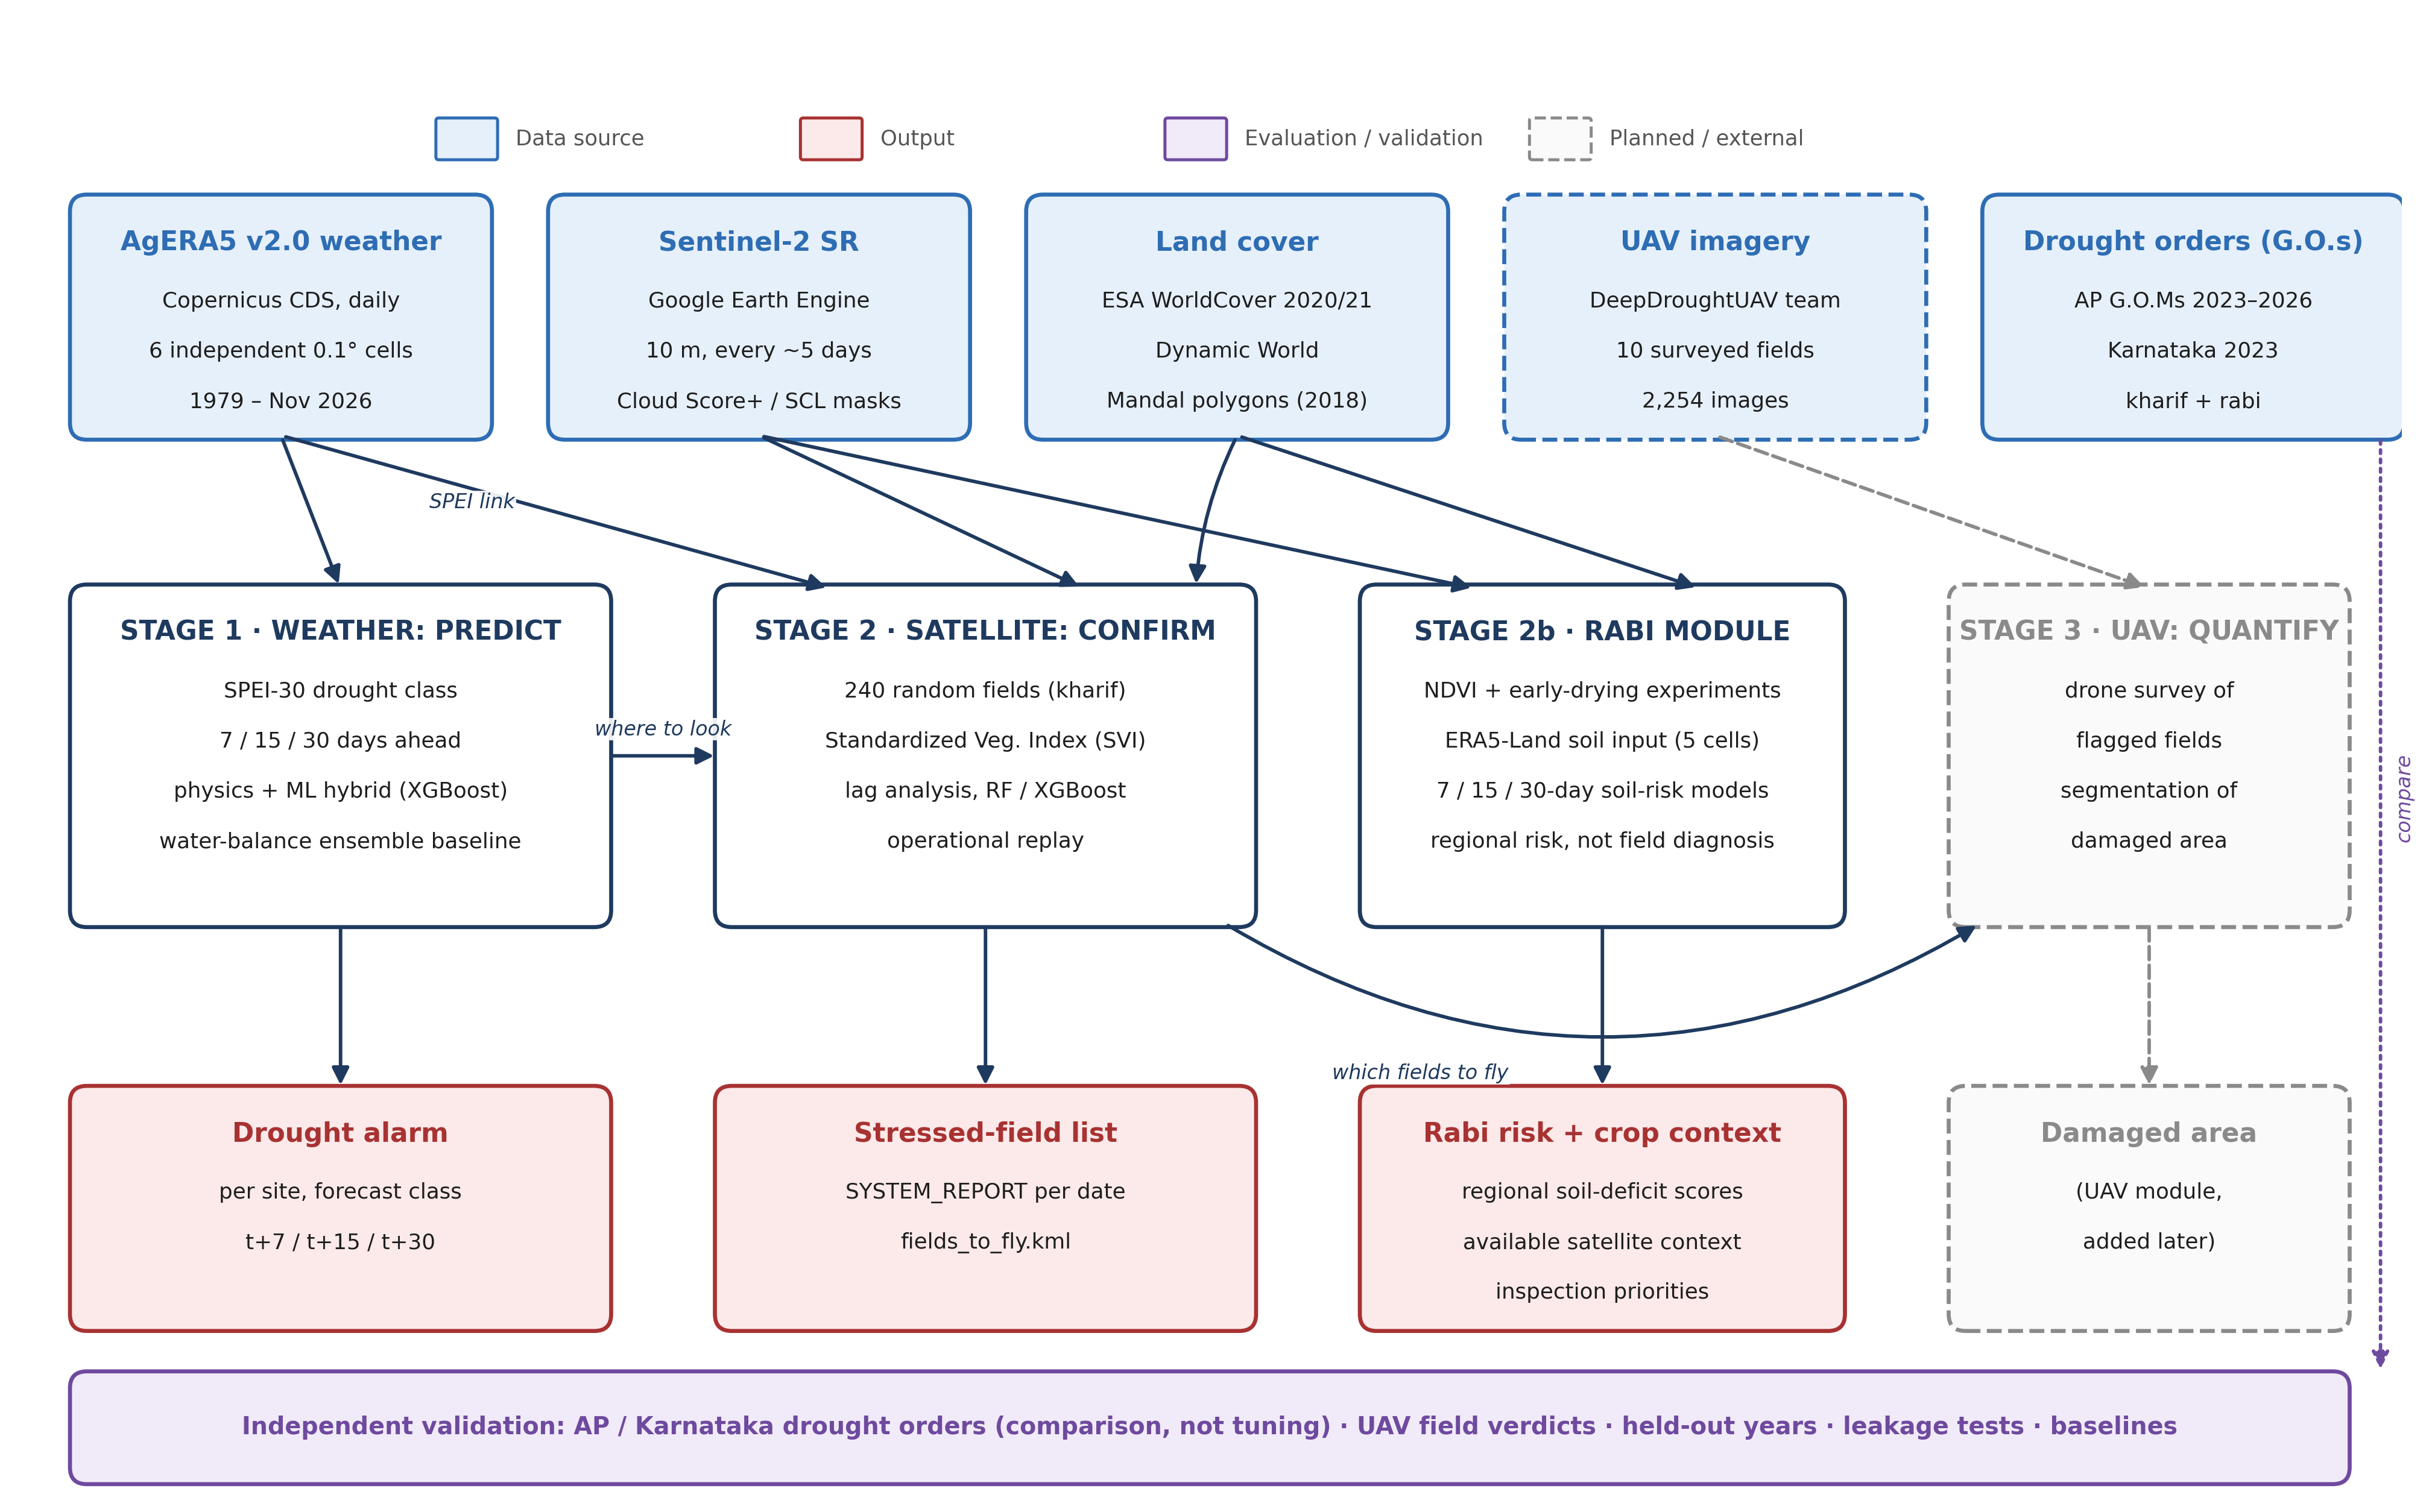
\includegraphics[width=0.97\textwidth]{figures/fig1_system_architecture.png}
\caption{Overall system architecture: weather (predict) $\rightarrow$ satellite (confirm) $\rightarrow$ UAV (quantify), with the separate rabi module and independent validation.}
\label{fig:system}
\end{figure}

\begin{figure}[H]
\centering
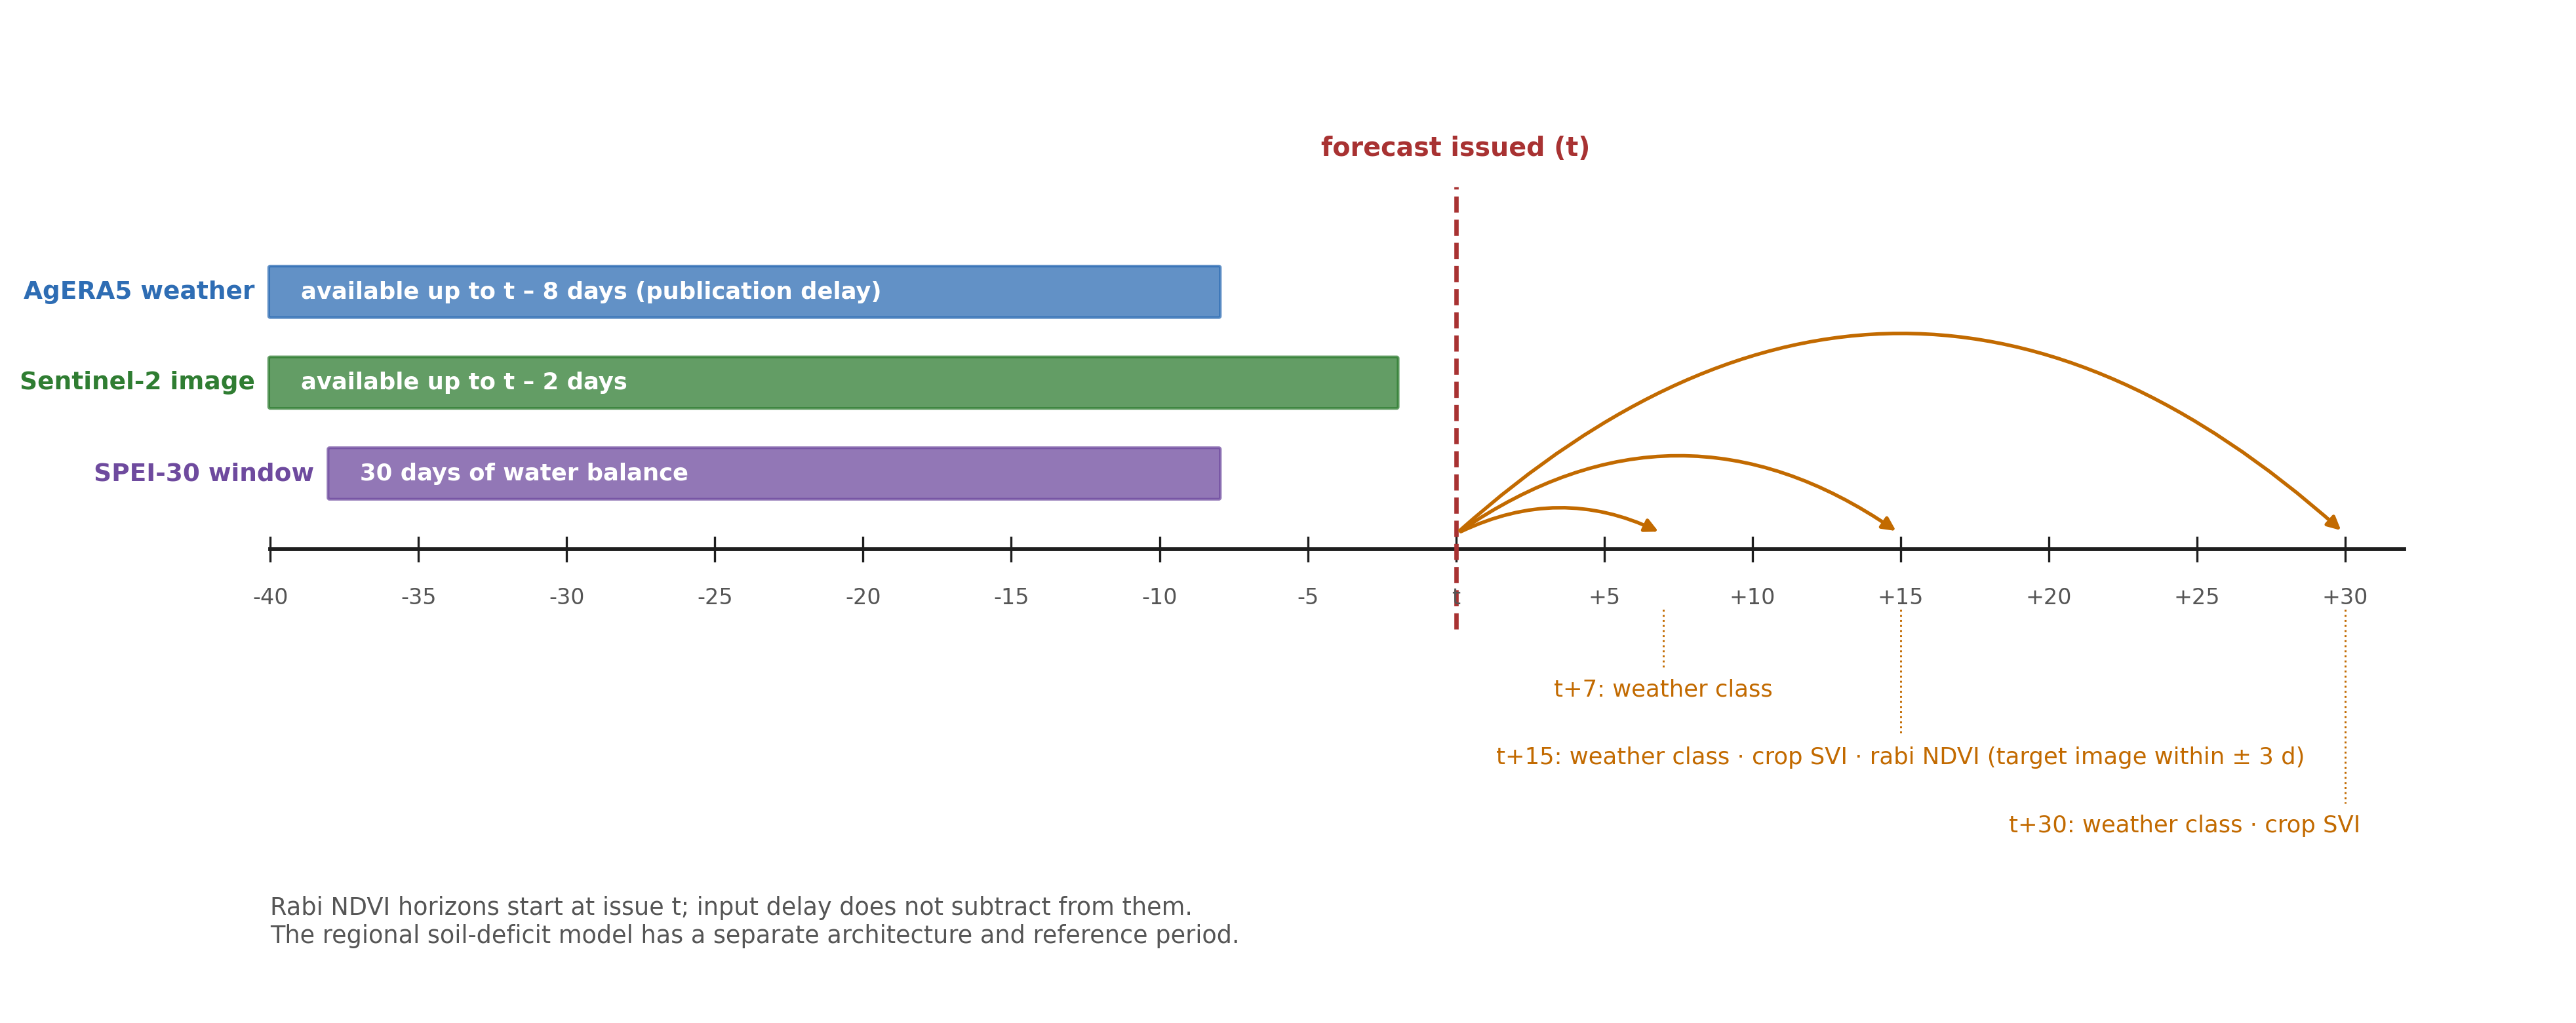
\includegraphics[width=0.92\textwidth]{figures/fig5_operational_timing.png}
\caption{Operational timing on forecast date $t$: data availability (publication delays) and forecast horizons.}
\label{fig:timing}
\end{figure}

\begin{figure}[H]
\centering
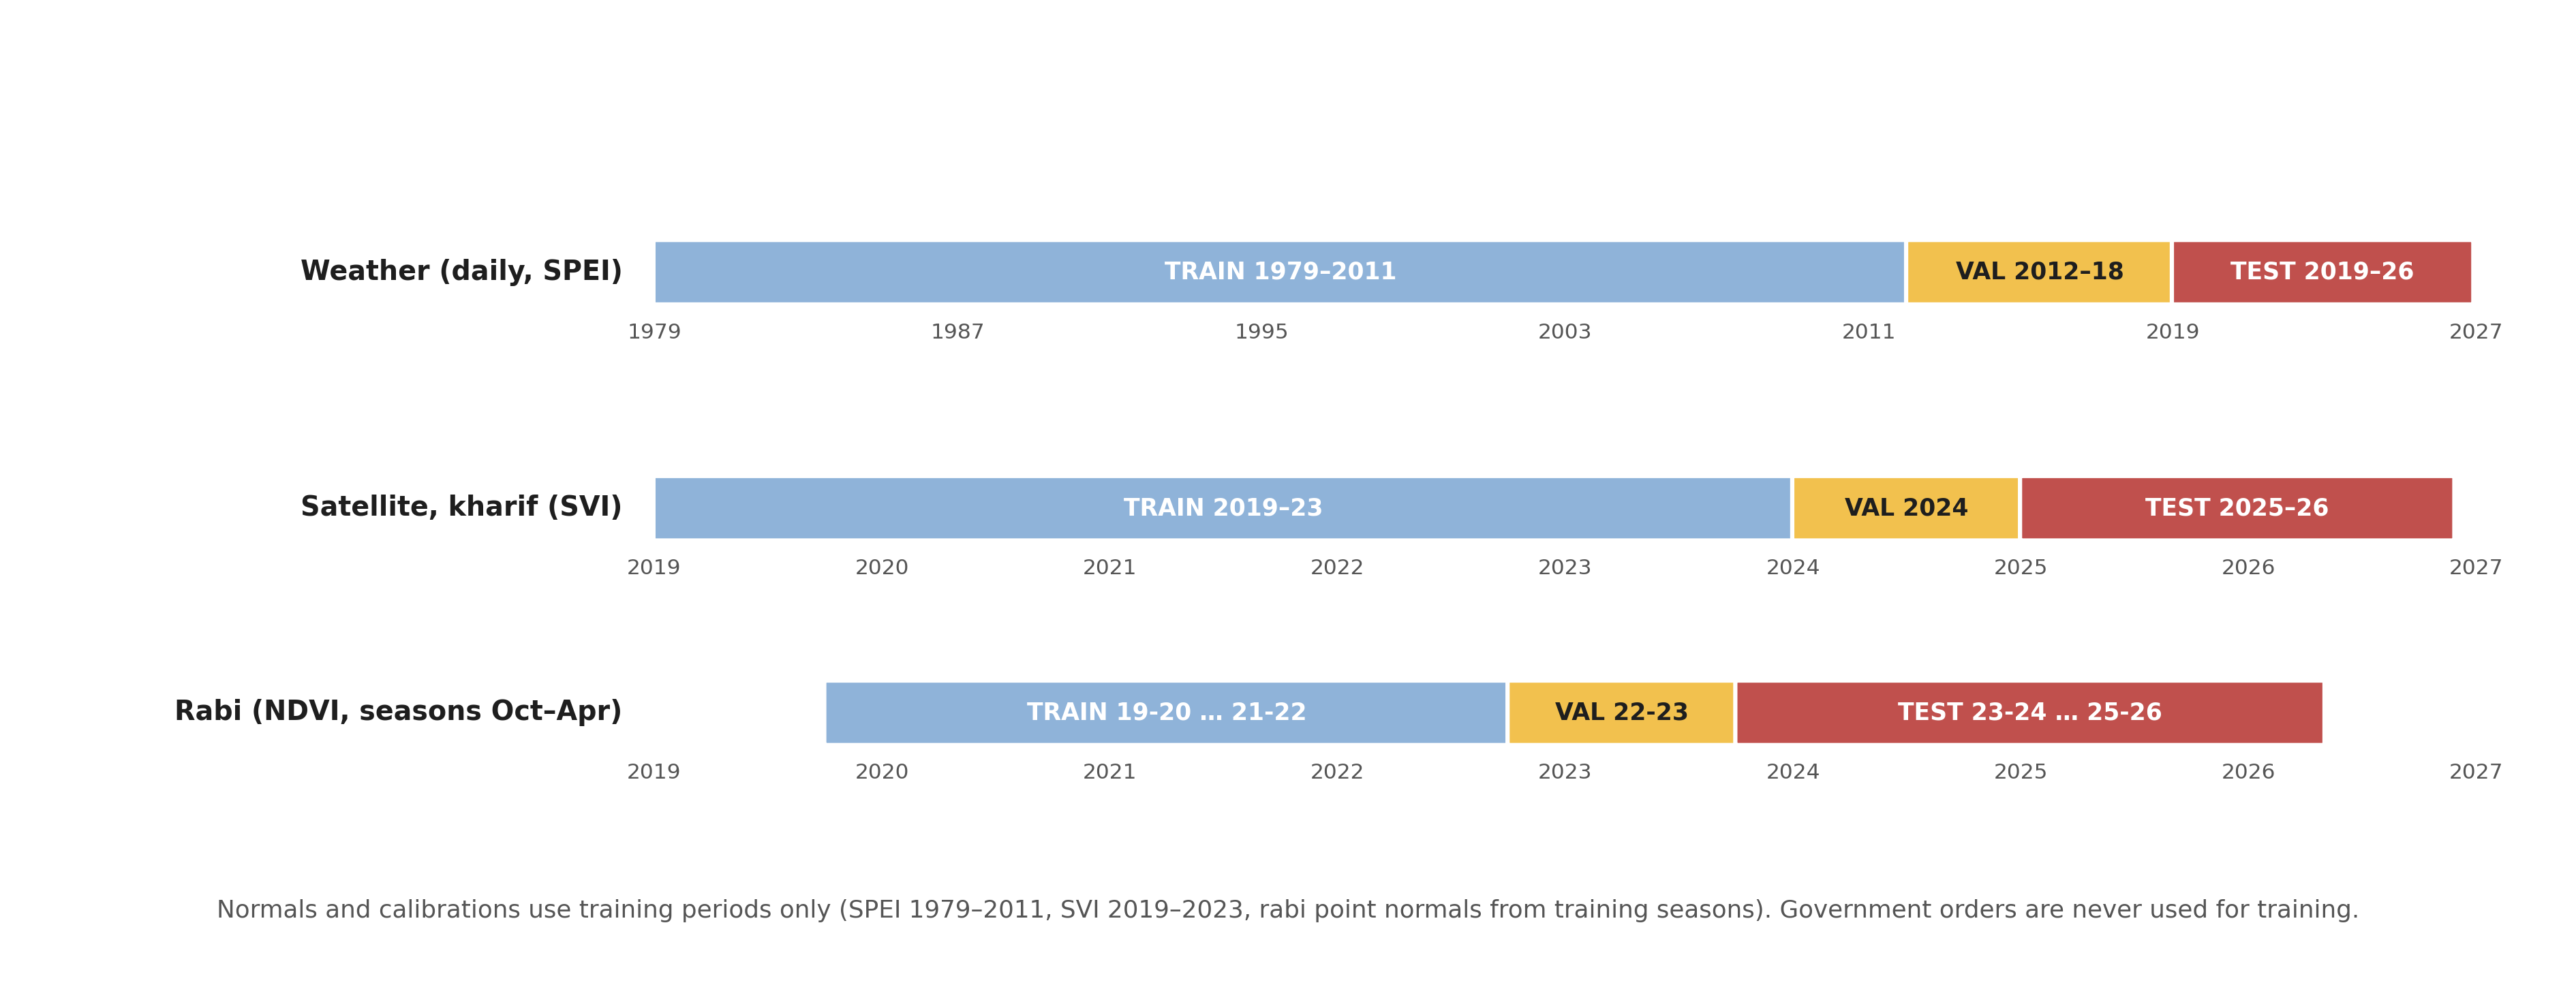
\includegraphics[width=0.92\textwidth]{figures/fig6_data_splits.png}
\caption{Training, validation and test periods of the three modules.}
\label{fig:splits}
\end{figure}

% ============================================================================
\section{Module 1: Weather Time-Series Drought Forecasting}

\subsection{Method}
\textbf{Labels.} For each site the daily water balance $D_t = P_t - \mathrm{ET}_{0,t}$ is accumulated over 30 days, $\mathrm{WB30}_t = \sum_{k=0}^{29} D_{t-k}$, and standardised to SPEI-30~\cite{vicente2010} with a log-logistic distribution fitted by L-moments per site and calendar month on \textbf{1979--2011 only}; the parameters are frozen. The target is the drought class on day $t+h$, $h \in \{7, 15, 30\}$.

\textbf{Inputs.} A 30-day window ($t-29 \dots t$) of features. Five feature sets are compared: \texttt{weather} (9 AgERA5 variables), \texttt{weather\_spei} (+ SPEI history up to $t$), \texttt{spei\_only}, \texttt{weather\_spei\_doy} (+ $\sin$/$\cos$ day of year) and the \textbf{hybrid} \texttt{weather\_spei\_doy\_wb}, which adds the three class probabilities of a physical water-balance ensemble.

\textbf{Water-balance ensemble (physics).} On day $t$ part of the 30-day SPEI window for $t+h$ is already observed; the unknown days are filled with each 1979--2011 year's water balance in turn, giving 33 possible SPEI values. The share of years in each class is a class probability:
\begin{equation}
\hat{p}_c = \frac{1}{|Y|}\sum_{y \in Y} \mathbf{1}\!\left[\text{class}\!\left(\mathrm{SPEI}^{(y)}_{t+h}\right) = c\right], \qquad Y = \{1979,\dots,2011\}.
\end{equation}

\textbf{Models.} Random Forest~\cite{breiman2001} and XGBoost~\cite{chen2016} (flattened $30 \times F$ input), LSTM and Transformer (sequence input), and a soft-voting ensemble weighted by validation \mf: $\hat{P} = \sum_m w_m P_m$, $\sum_m w_m = 1$. Five seeds each. Baselines: persistence (class today), Markov transition, climatology, majority class and the water-balance ensemble.

\textbf{Evaluation.} A purged chronological split (TRAIN 1979--2011, VAL 2012--2018, TEST 2019--2026); a sample is kept only if its whole span lies in one period. Scalers, early stopping, ensemble weights and model selection use TRAIN/VAL only. Metrics: \mf, balanced accuracy, ROC-AUC, block-bootstrap 95\,\% confidence intervals, leave-one-cluster-out (Kurnool vs south) and the Marusov et al.~\cite{marusov2024} protocol. 22 automated tests check integrity and leakage.

\begin{figure}[H]
\centering
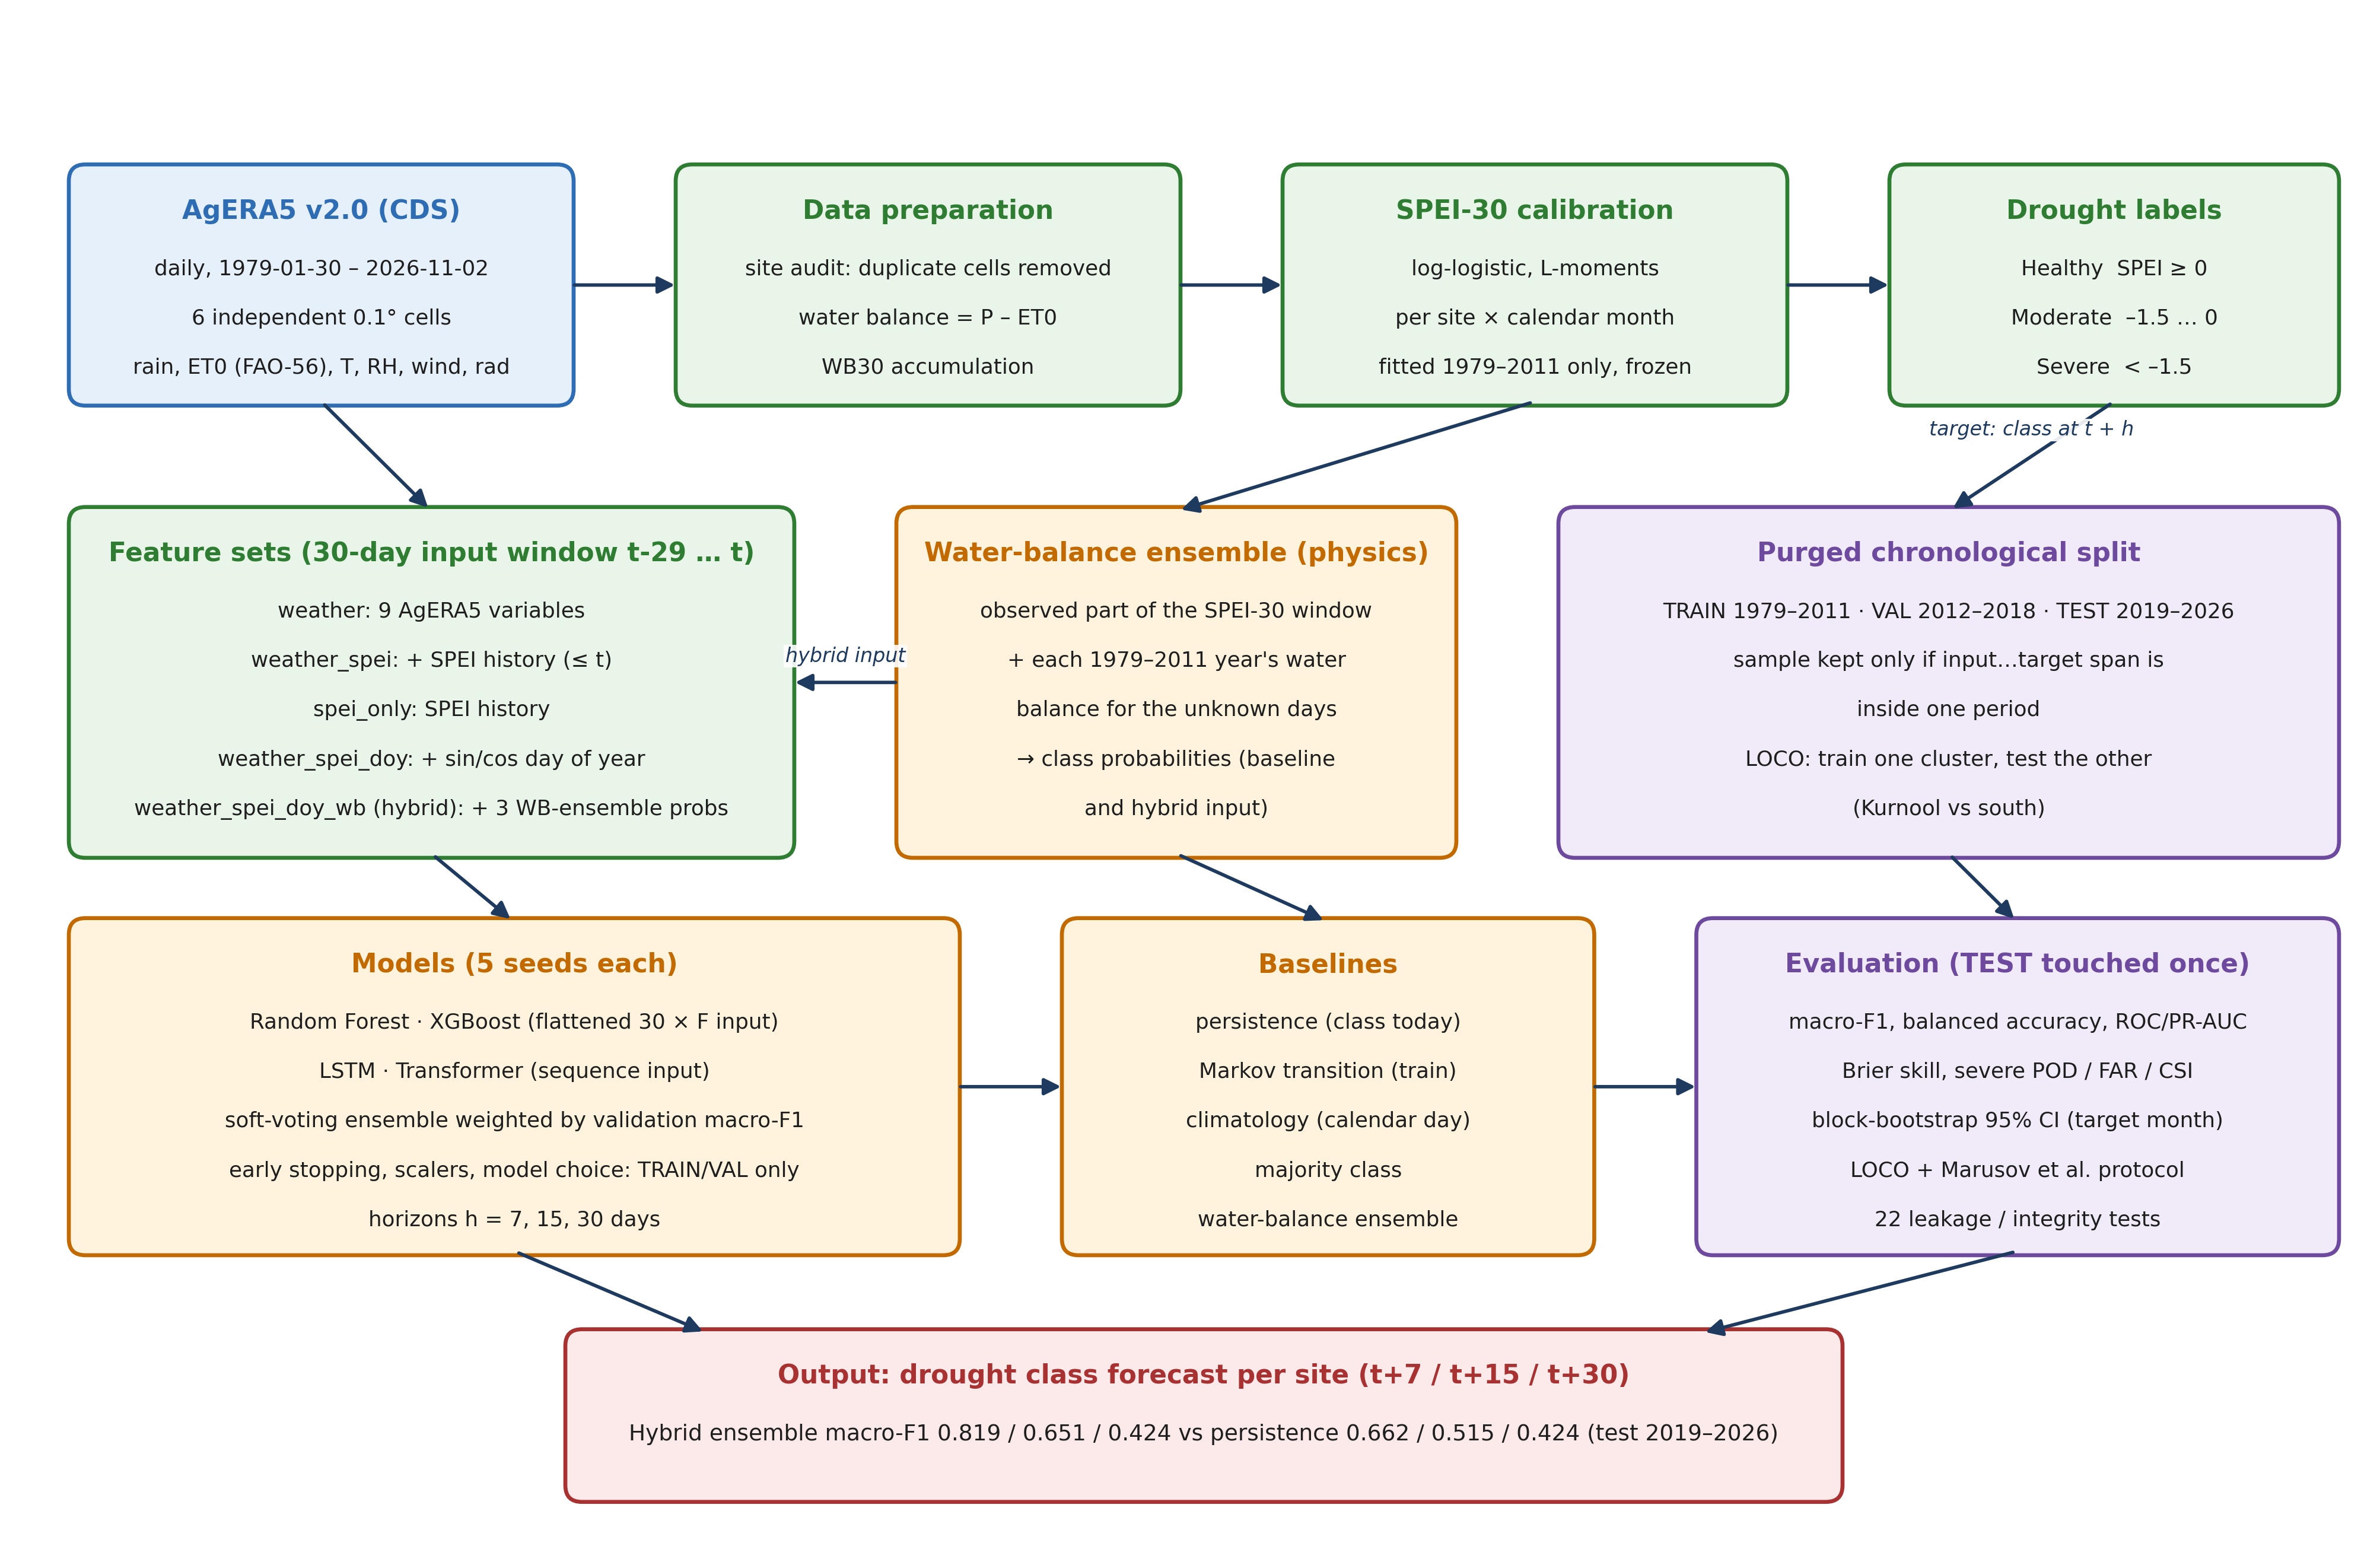
\includegraphics[width=0.95\textwidth]{figures/fig2_weather_module_architecture.png}
\caption{Weather module architecture.}
\label{fig:weather_arch}
\end{figure}

\subsection{Results}

\subsubsection{Overall skill and comparison with baselines}
Table~\ref{tab:w_models} compares all four models and their ensemble with five baselines on the test years 2019--2026 (about 17,000 forecasts per horizon, all sites). Every model beats persistence clearly at 7 and 15 days; the soft-voting ensemble is best at every horizon. Seed-to-seed variation is small ($\le 0.016$), so the ranking is stable. Markov transition, climatology and the majority class are far weaker, showing that the problem is not trivial.

% --- table w_models (generated by make_results.py)
\begin{table}[H]
\centering
\caption{Weather module: \mf{} of every model with the hybrid inputs and of every baseline (test 2019--2026, all sites; mean $\pm$ s.d.\ over 5 seeds).}
\label{tab:w_models}
\small
\begin{tabular}{@{}lccc@{}}
\toprule
\textbf{Model} & \textbf{7 days} & \textbf{15 days} & \textbf{30 days} \\
\midrule
Persistence & 0.662 & 0.515 & 0.424 \\
Markov transition & 0.493 & 0.424 & 0.377 \\
Climatology & 0.309 & 0.310 & 0.310 \\
Majority class & 0.261 & 0.261 & 0.261 \\
Water-balance ensemble (physics) & 0.783 & 0.592 & 0.375 \\
\midrule
Random Forest & 0.775 $\pm$ 0.002 & 0.617 $\pm$ 0.004 & 0.383 $\pm$ 0.001 \\
XGBoost & 0.814 $\pm$ 0.003 & 0.631 $\pm$ 0.002 & 0.418 $\pm$ 0.003 \\
LSTM & 0.806 $\pm$ 0.006 & 0.642 $\pm$ 0.008 & 0.406 $\pm$ 0.014 \\
Transformer & 0.809 $\pm$ 0.005 & 0.650 $\pm$ 0.016 & 0.407 $\pm$ 0.011 \\
\textbf{Soft-voting ensemble} & \textbf{0.819 $\pm$ 0.003} & \textbf{0.651 $\pm$ 0.009} & \textbf{0.424 $\pm$ 0.012} \\
\bottomrule
\end{tabular}
\end{table}


\begin{figure}[H]
\centering
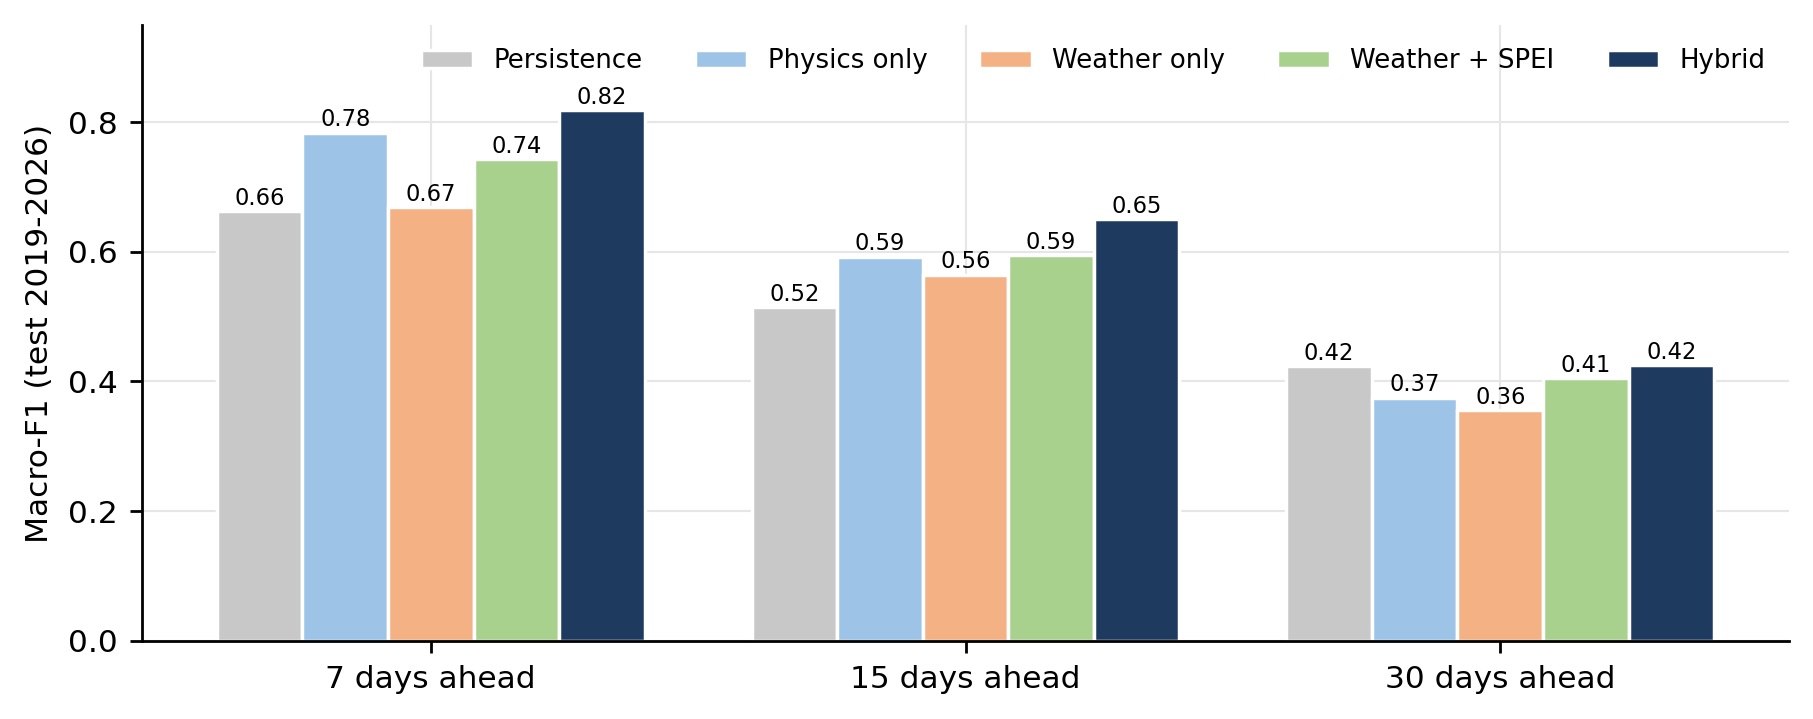
\includegraphics[width=0.85\textwidth]{figures/res_w_bars.png}
\caption{Weather module \mf{} on test years 2019--2026: persistence, the physical water-balance ensemble, and the ensemble model with three input sets.}
\label{fig:w_bars}
\end{figure}

\subsubsection{Which inputs matter}
Table~\ref{tab:w_features} adds the inputs one group at a time. Weather alone barely beats persistence (0.668 vs 0.662 at 7 days). Adding the SPEI history gives +0.075, the day of year a further +0.013, and the water-balance ensemble probabilities the largest single gain (+0.063 at 7 days, +0.039 at 15 days). The physical knowledge of how much of the future SPEI window is already fixed is therefore the most valuable input --- the hybrid design is justified by the data, not assumed.

% --- table w_features (generated by make_results.py)
\begin{table}[H]
\centering
\caption{Weather module: effect of the input feature set (\mf{} of the soft-voting ensemble, test 2019--2026).}
\label{tab:w_features}
\small
\begin{tabular}{@{}lccc@{}}
\toprule
\textbf{Inputs} & \textbf{7 days} & \textbf{15 days} & \textbf{30 days} \\
\midrule
Weather only (9 AgERA5 variables) & 0.668 & 0.565 & 0.356 \\
SPEI history only & 0.694 & 0.530 & 0.377 \\
Weather + SPEI history & 0.743 & 0.594 & 0.405 \\
+ day of year & 0.756 & 0.612 & 0.406 \\
\textbf{+ water-balance probabilities (hybrid)} & \textbf{0.819} & \textbf{0.651} & \textbf{0.424} \\
Persistence (reference) & 0.662 & 0.515 & 0.424 \\
\bottomrule
\end{tabular}
\end{table}


\begin{table}[H]
\centering
\caption{Weather module, test years 2019--2026, all sites (\mf{} unless stated).}
\label{tab:weather}
\small
\begin{tabular}{@{}lccc@{}}
\toprule
\textbf{Model} & \textbf{7 days} & \textbf{15 days} & \textbf{30 days} \\
\midrule
Persistence (no change) & 0.662 & 0.515 & 0.424 \\
Water-balance ensemble (physics only) & 0.783 & 0.592 & 0.375 \\
Best model without physics (XGBoost) & 0.755 & 0.613 & 0.424 \\
\textbf{Hybrid, ensemble of 4 models} & \textbf{0.819} & \textbf{0.651} & 0.424 \\
Hybrid vs physics, $\Delta$ [95\,\% CI] & [$-0.007$, $+0.088$] & [$+0.010$, $+0.099$] & [$+0.023$, $+0.084$] \\
Balanced accuracy, hybrid & 85.6\,\% & 68.3\,\% & 42.5\,\% \\
ROC-AUC, hybrid & 0.97 & 0.90 & 0.68 \\
\bottomrule
\end{tabular}
\end{table}

The hybrid also beats the physical model alone (Table~\ref{tab:weather}): significantly at 15 days ([+0.010, +0.099]) and at 30 days, but not at 7 days, where physics is already very strong (0.783).

\subsubsection{Severe drought warning and confusion between classes}
For early warning the severe class matters most. With a threshold tuned on validation years only, the ensemble detects 80\,\% of severe days 7 days ahead (POD 0.80, false-alarm ratio 0.34) and 61\,\% at 15 days, against a severe F1 of 0.52 / 0.33 for persistence (Table~\ref{tab:w_severe}). The Brier skill score is clearly positive at 7 and 15 days and close to zero at 30 days. The confusion matrices (Fig.~\ref{fig:w_conf}) show that almost all errors are between neighbouring classes: at 7 days no severe day is predicted as healthy and only 16 of 10,908 healthy days are predicted severe.

% --- table w_severe (generated by make_results.py)
\begin{table}[H]
\centering
\caption{Weather module: severe-drought warning and probabilistic skill of the hybrid ensemble (test 2019--2026). POD / FAR / CSI at a severe-probability threshold tuned on validation; BSS = Brier skill score vs climatology.}
\label{tab:w_severe}
\footnotesize
\begin{tabular}{@{}lccccccc@{}}
\toprule
\textbf{Horizon} & \textbf{Severe F1} & \textbf{POD} & \textbf{FAR} & \textbf{CSI} & \textbf{ROC-AUC} & \textbf{BSS} & \textbf{Severe F1 persistence} \\
\midrule
7 days & 0.724 & 0.80 & 0.34 & 0.57 & 0.966 & +0.67 & 0.524 \\
15 days & 0.444 & 0.61 & 0.62 & 0.30 & 0.903 & +0.43 & 0.326 \\
30 days & 0.141 & 0.32 & 0.86 & 0.10 & 0.684 & +0.06 & 0.185 \\
\bottomrule
\end{tabular}
\end{table}


\begin{figure}[H]
\centering
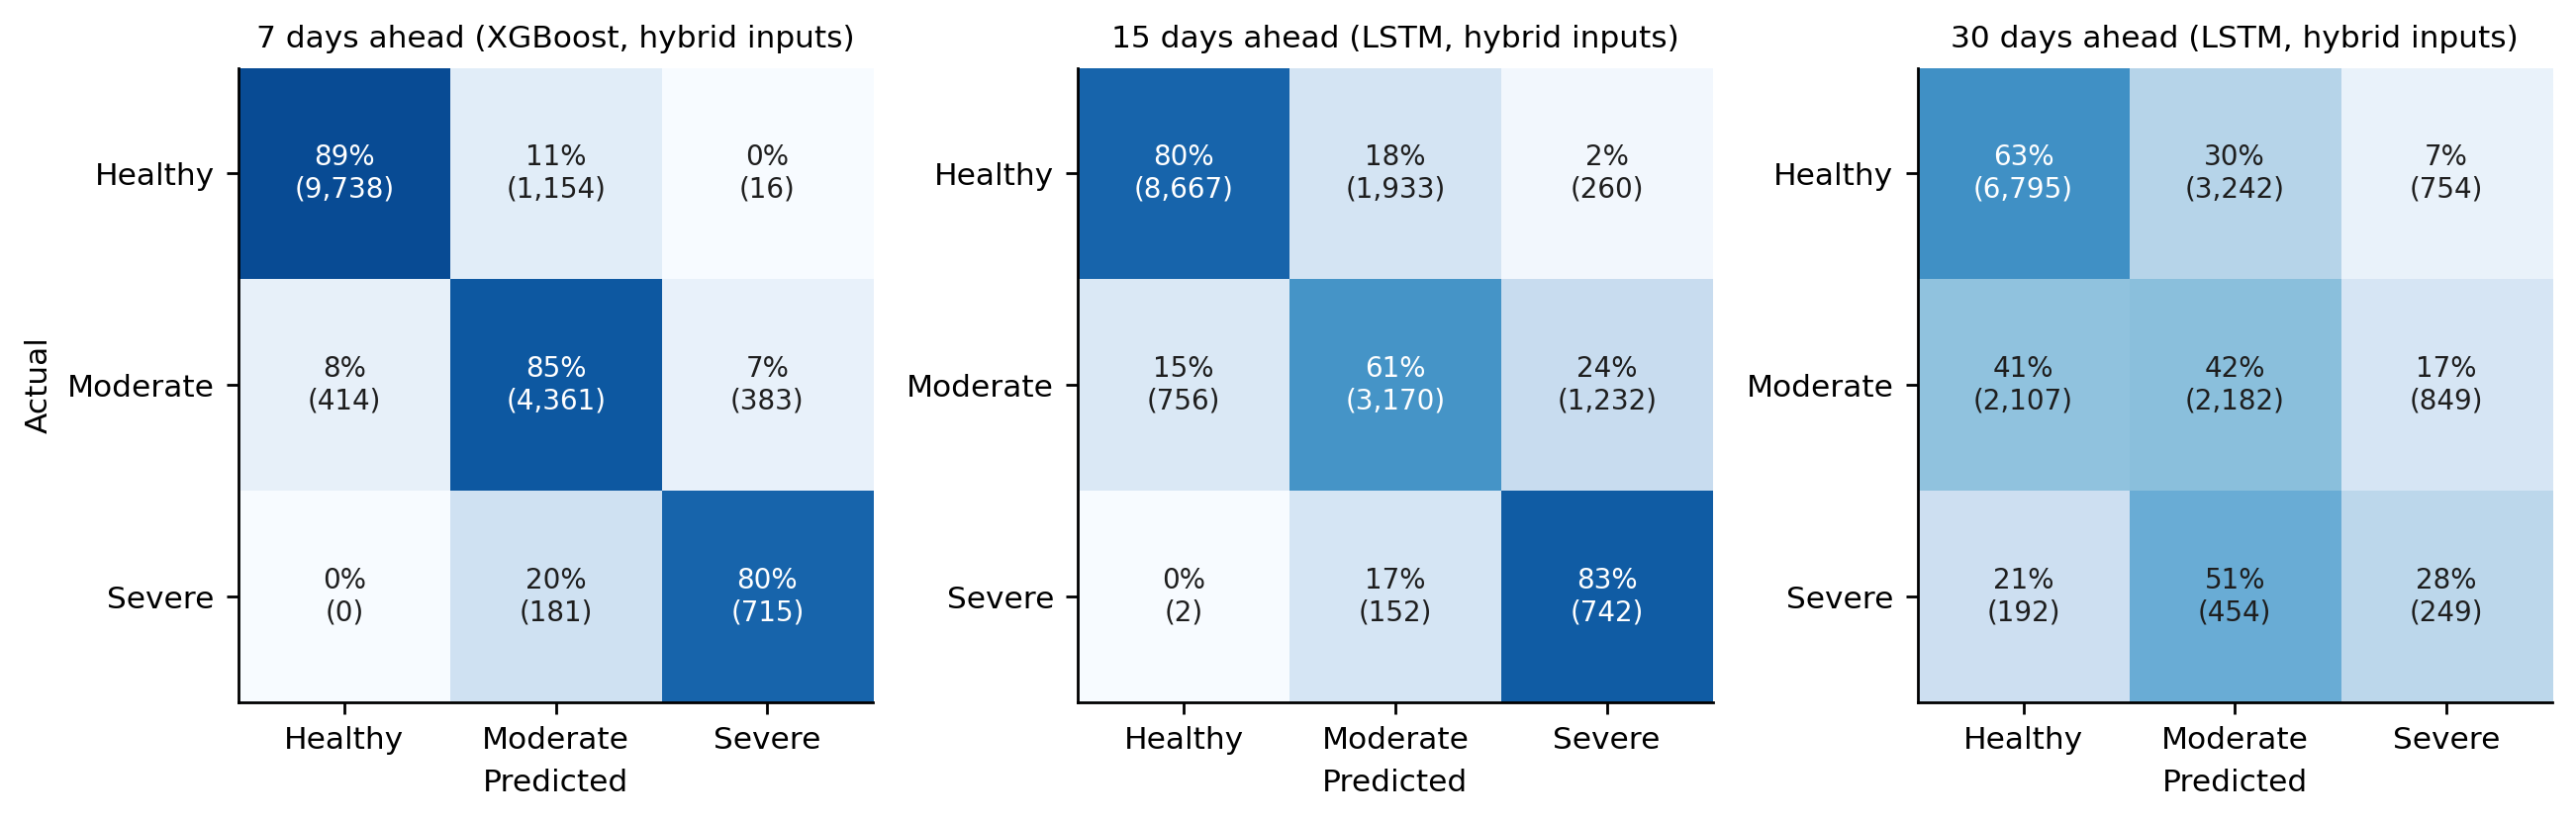
\includegraphics[width=0.97\textwidth]{figures/res_w_confusion.png}
\caption{Row-normalised confusion matrices of the best hybrid model at each horizon (test 2019--2026, all sites).}
\label{fig:w_conf}
\end{figure}

\subsubsection{Unseen regions and a published protocol}
To test spatial transfer, models were trained on one region and tested on the other region's 2019--2026 data (Table~\ref{tab:w_loco}). The hybrid ensemble keeps its skill (0.826 / 0.640 for Kurnool, 0.796 / 0.627 for the south at 7 / 15 days), while the ensemble without physics inputs drops close to persistence --- the physics input is what makes the model transferable. Under the Marusov et al.~\cite{marusov2024} protocol (Table~\ref{tab:w_marusov}), weather inputs raise the 15-day median ROC-AUC from 0.81 (SPEI history) to 0.89; at 30 days a logistic regression on the last SPEI value is as good as any deep model.

% --- table w_loco (generated by make_results.py)
\begin{table}[H]
\centering
\caption{Weather module, leave-one-cluster-out: trained on one region, tested on the other region's 2019--2026 data (\mf).}
\label{tab:w_loco}
\footnotesize
\begin{tabular}{@{}llccc@{}}
\toprule
\textbf{Test region} & \textbf{Model} & \textbf{7 days} & \textbf{15 days} & \textbf{30 days} \\
\midrule
Train south $\rightarrow$ test Kurnool & Persistence & 0.658 & 0.479 & 0.440 \\
 & Water-balance ensemble & 0.810 & 0.643 & 0.382 \\
 & Ensemble, weather + SPEI & 0.682 & 0.518 & 0.346 \\
 & Ensemble, hybrid & 0.826 & 0.640 & 0.338 \\
\midrule
Train Kurnool $\rightarrow$ test south & Persistence & 0.663 & 0.541 & 0.407 \\
 & Water-balance ensemble & 0.760 & 0.547 & 0.367 \\
 & Ensemble, weather + SPEI & 0.653 & 0.529 & 0.348 \\
 & Ensemble, hybrid & 0.796 & 0.627 & 0.424 \\
\bottomrule
\end{tabular}
\end{table}

% --- table w_marusov (generated by make_results.py)
\begin{table}[H]
\centering
\caption{Weather module under the Marusov et al.\ protocol (binary drought SPEI $< -1$; median ROC-AUC over sites).}
\label{tab:w_marusov}
\footnotesize
\begin{tabular}{@{}lccc@{}}
\toprule
\textbf{Model and input} & \textbf{7 days} & \textbf{15 days} & \textbf{30 days} \\
\midrule
Persistence & 0.778 & 0.687 & 0.598 \\
Logistic regression on last SPEI & 0.918 & 0.806 & 0.701 \\
XGBoost, SPEI history & 0.919 & 0.777 & 0.587 \\
LSTM, SPEI history & 0.939 & 0.809 & 0.682 \\
\textbf{XGBoost, weather + SPEI} & \textbf{0.960} & \textbf{0.886} & \textbf{0.706} \\
LSTM, weather + SPEI & 0.949 & 0.873 & 0.575 \\
\bottomrule
\end{tabular}
\end{table}


\textbf{Corrections made during development.} An internal audit of the first version found a duplicate weather cell counted as two sites, SPEI standardised on all years (test information in the labels), a 1-day horizon already solved by persistence, samples crossing split boundaries, and two sites on the wrong weather cell. All were fixed before the results above were produced; the earlier, higher scores (e.g.\ \mf{} above 0.85) are not valid and are not reported.

% ============================================================================
\section{Module 2: Satellite Drought Confirmation (Kharif)}

\subsection{Method}
\textbf{Farmland and fields.} No surveyed field boundaries exist, so farmland is mapped automatically in Google Earth Engine from training years only: ESA WorldCover cropland within 3\,km of each site, minus Dynamic World built-up, tree and water pixels, keeping pixels with a crop cycle in at least 2 years. SNIC superpixels~\cite{achanta2017} split the farmland into 13,750 field segments of 0.3--10\,ha. A seeded random sample of 20 rainfed and 10 irrigated segments per site gives \textbf{240 fields}; irrigated = green in March--May in at least 3 years.

\textbf{Time series.} Every Sentinel-2 image is kept for a field if at least 60\,\% of its pixels are clear. Series are placed on a 5-day grid in three versions: \emph{causal} (last observation carried forward; the only model input), \emph{interpolated} (labels only) and \emph{reference} (normals).

\textbf{Label.} The Standardized Vegetation Index~\cite{peters2002},
\begin{equation}
\mathrm{SVI}_{f,d} = \frac{\mathrm{NDVI}_{f,d} - \mu_{f,\mathrm{doy}(d)}}{\sigma_{f,\mathrm{doy}(d)}},
\end{equation}
per field $f$ and day of year, with mean ($\pm 15$ days) and spread ($\pm 30$ days) from images up to 31 Dec 2023 and the scored year removed. Classes use the SPEI thresholds (0, $-1.5$). VCI~\cite{kogan1995} is kept as an input only, because with 4--5 reference years about 20\,\% of dates get VCI $\approx 0$ by chance.

\textbf{Analyses.} (i) Lag analysis of SVI against SPEI-$k$ at lags 0--90 days, chosen on 2019--2023 and measured on 2024--2026. (ii) A crop-condition forecast of the SVI class 15 / 30 days ahead with RF and XGBoost in four versions: satellite history; + past weather; + weather-module forecast (the integrated system); + actual future weather (upper bound). TRAIN 2019--2023, VAL 2024, TEST 2025--2026, 5 seeds. (iii) An \textbf{operational replay} without any trained model: issued every 5 days from 1 June to 30 November with weather 7 days late and satellite 2 days late; \emph{alarm} = SPEI-30 $< -1$ or a severe +15-day forecast; \emph{confirmed} = median rainfed SVI $< -1$ from at least 5 clear fields.

\begin{figure}[H]
\centering
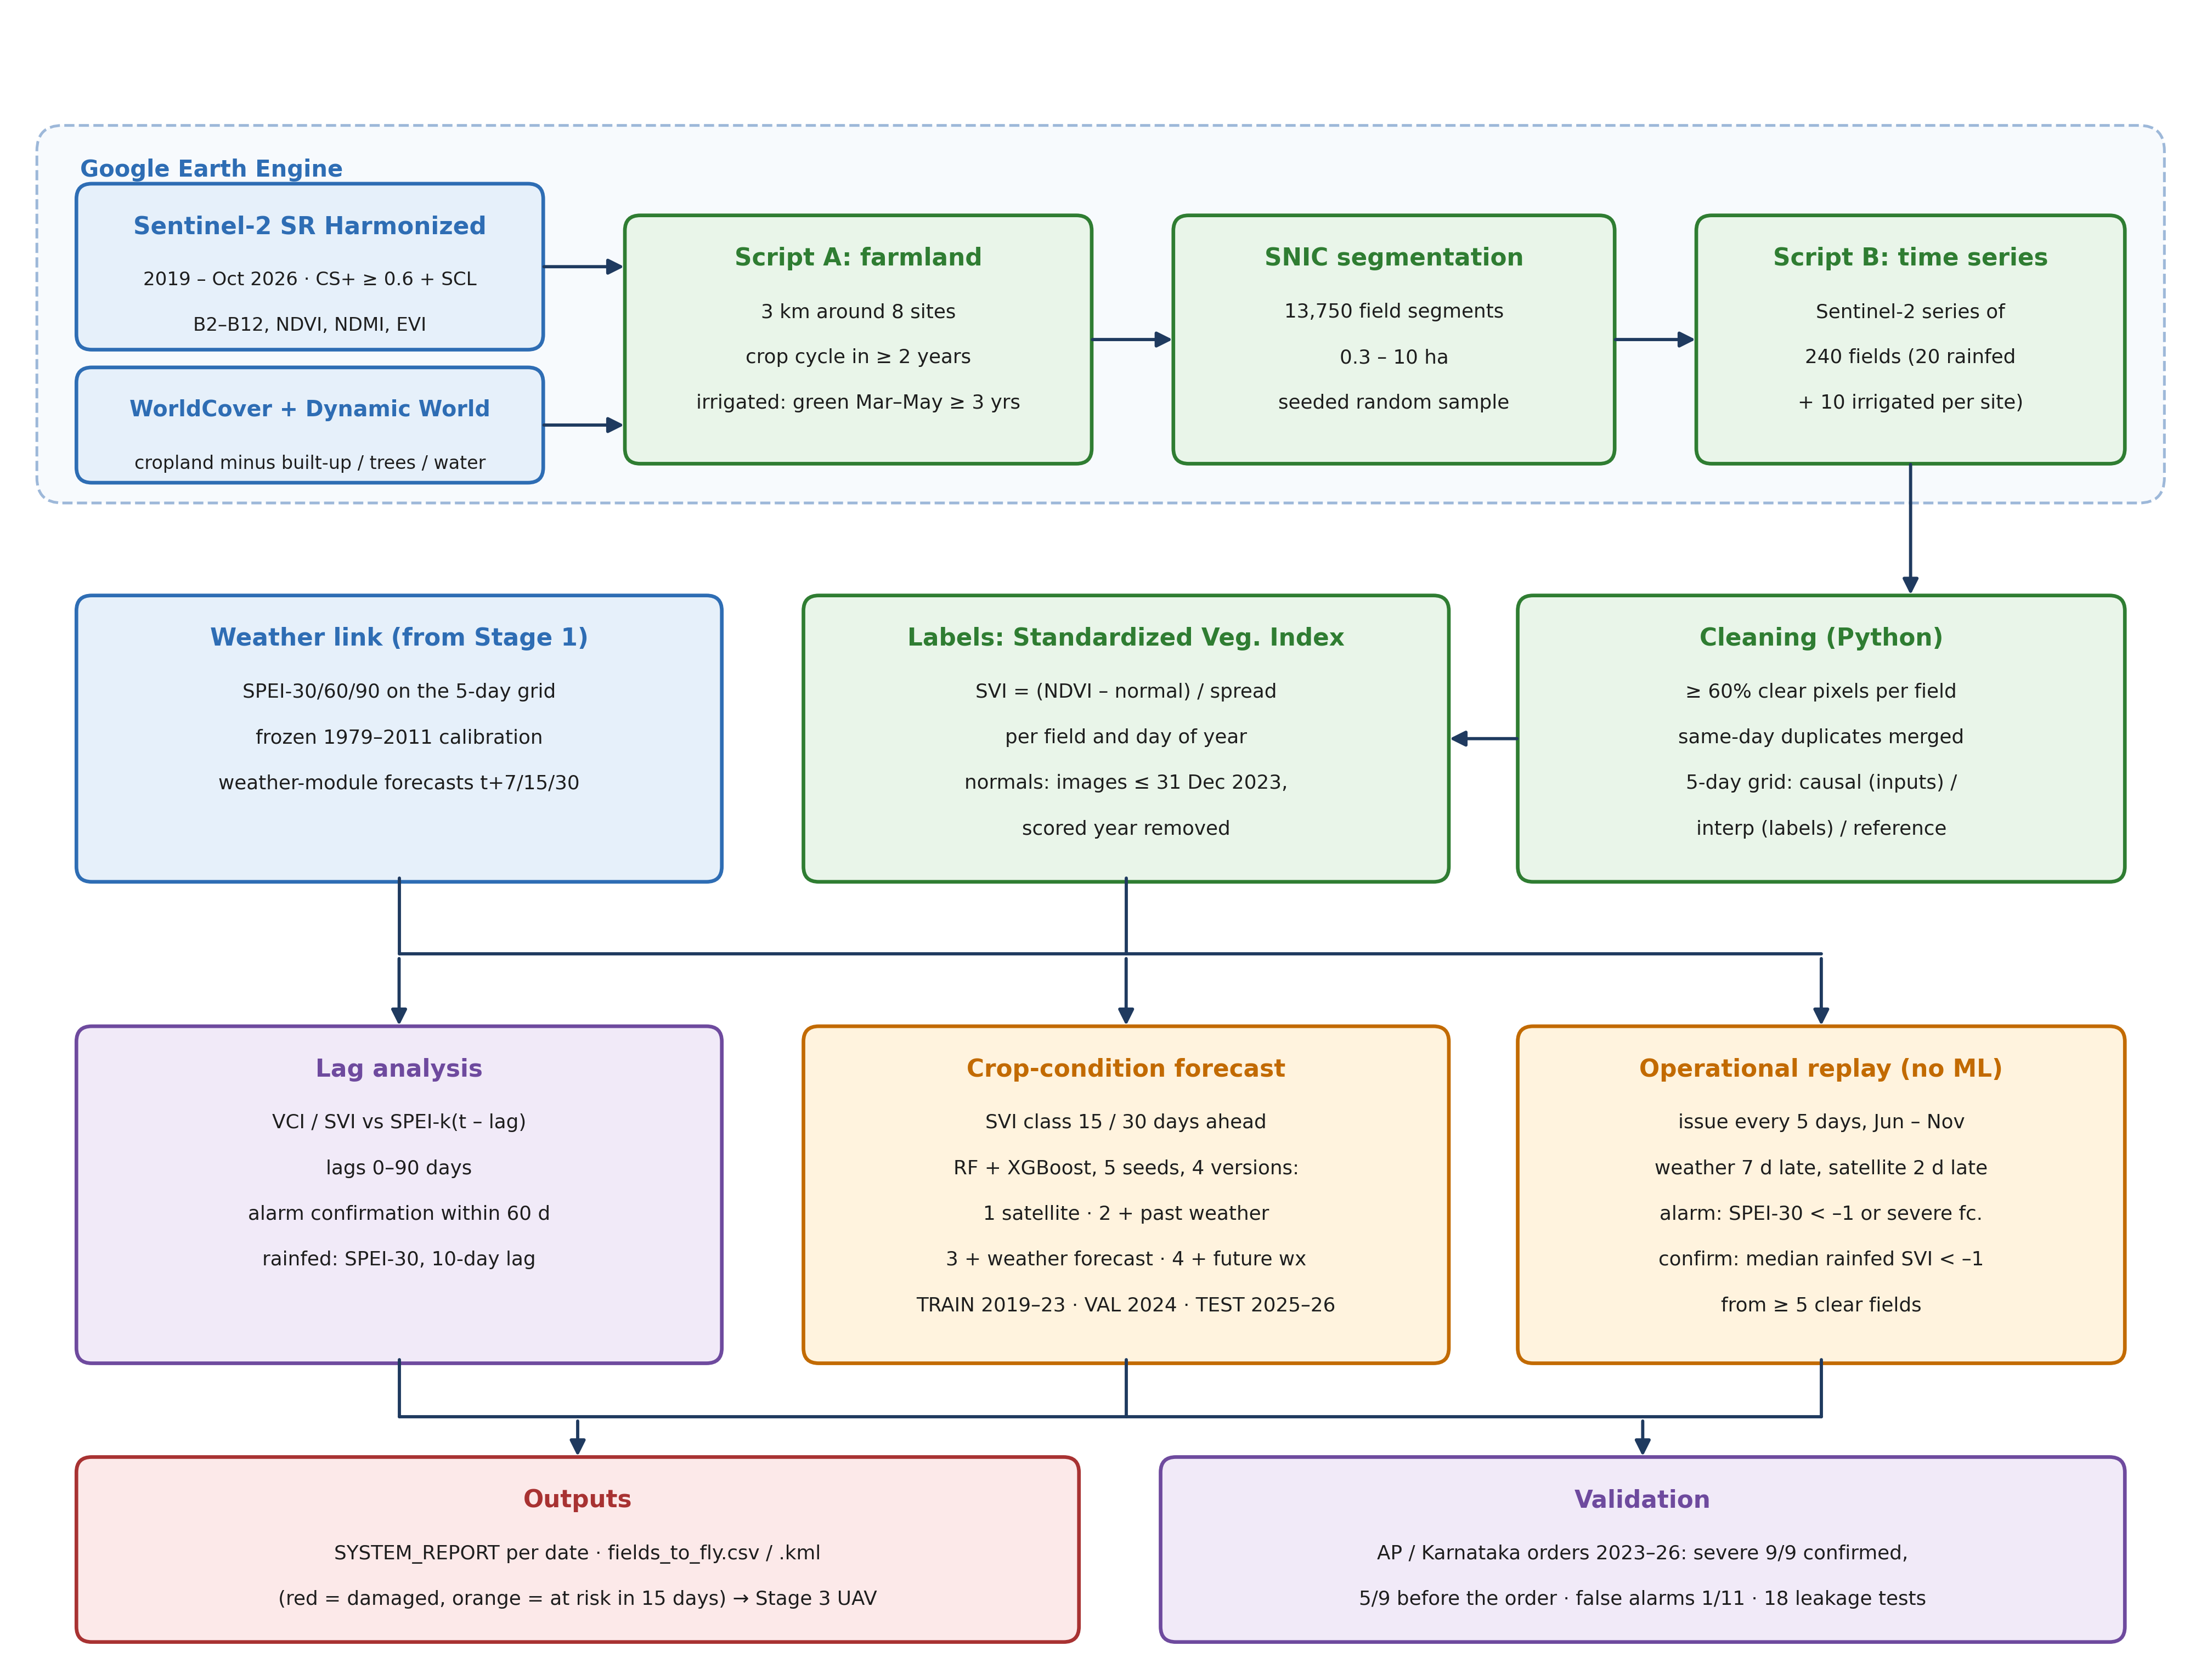
\includegraphics[width=0.95\textwidth]{figures/fig3_satellite_module_architecture.png}
\caption{Satellite module (kharif) architecture.}
\label{fig:sat_arch}
\end{figure}

\subsection{Results}

\subsubsection{Crops follow weather drought within about 10 days}
The SPEI scale and lag were chosen on 2019--2023 only and then measured on the unseen years 2024--2026 (Table~\ref{tab:s_lag}). On rainfed fields crop SVI follows SPEI-30 with a 10-day lag; the correlation hardly drops on the unseen years (0.48 $\rightarrow$ 0.45). Irrigated fields respond more weakly and to a longer, 60-day water balance, as expected when part of the water comes from irrigation. Figure~\ref{fig:s_lag} shows the full lag curves over 2019--2026: correlations are highest at short lags (0--15 days) for all SPEI scales and fall steadily beyond 20 days.

% --- table s_lag (generated by make_results.py)
\begin{table}[H]
\centering
\caption{Weather-to-crop lag: SPEI scale and lag chosen on 2019--2023 only, then measured on the unseen years 2024--2026 (Spearman $\rho$ between crop SVI and lagged SPEI, median over sites).}
\label{tab:s_lag}
\footnotesize
\begin{tabular}{@{}lcccc@{}}
\toprule
\textbf{Fields} & \textbf{SPEI scale} & \textbf{Lag} & \textbf{$\rho$ 2019--2023} & \textbf{$\rho$ 2024--2026 (range)} \\
\midrule
Rainfed & SPEI-30 & 10 days & 0.48 & 0.45 (0.16--0.58) \\
Irrigated & SPEI-60 & 15 days & 0.24 & 0.29 (0.12--0.46) \\
\bottomrule
\end{tabular}
\end{table}


\begin{figure}[H]
\centering
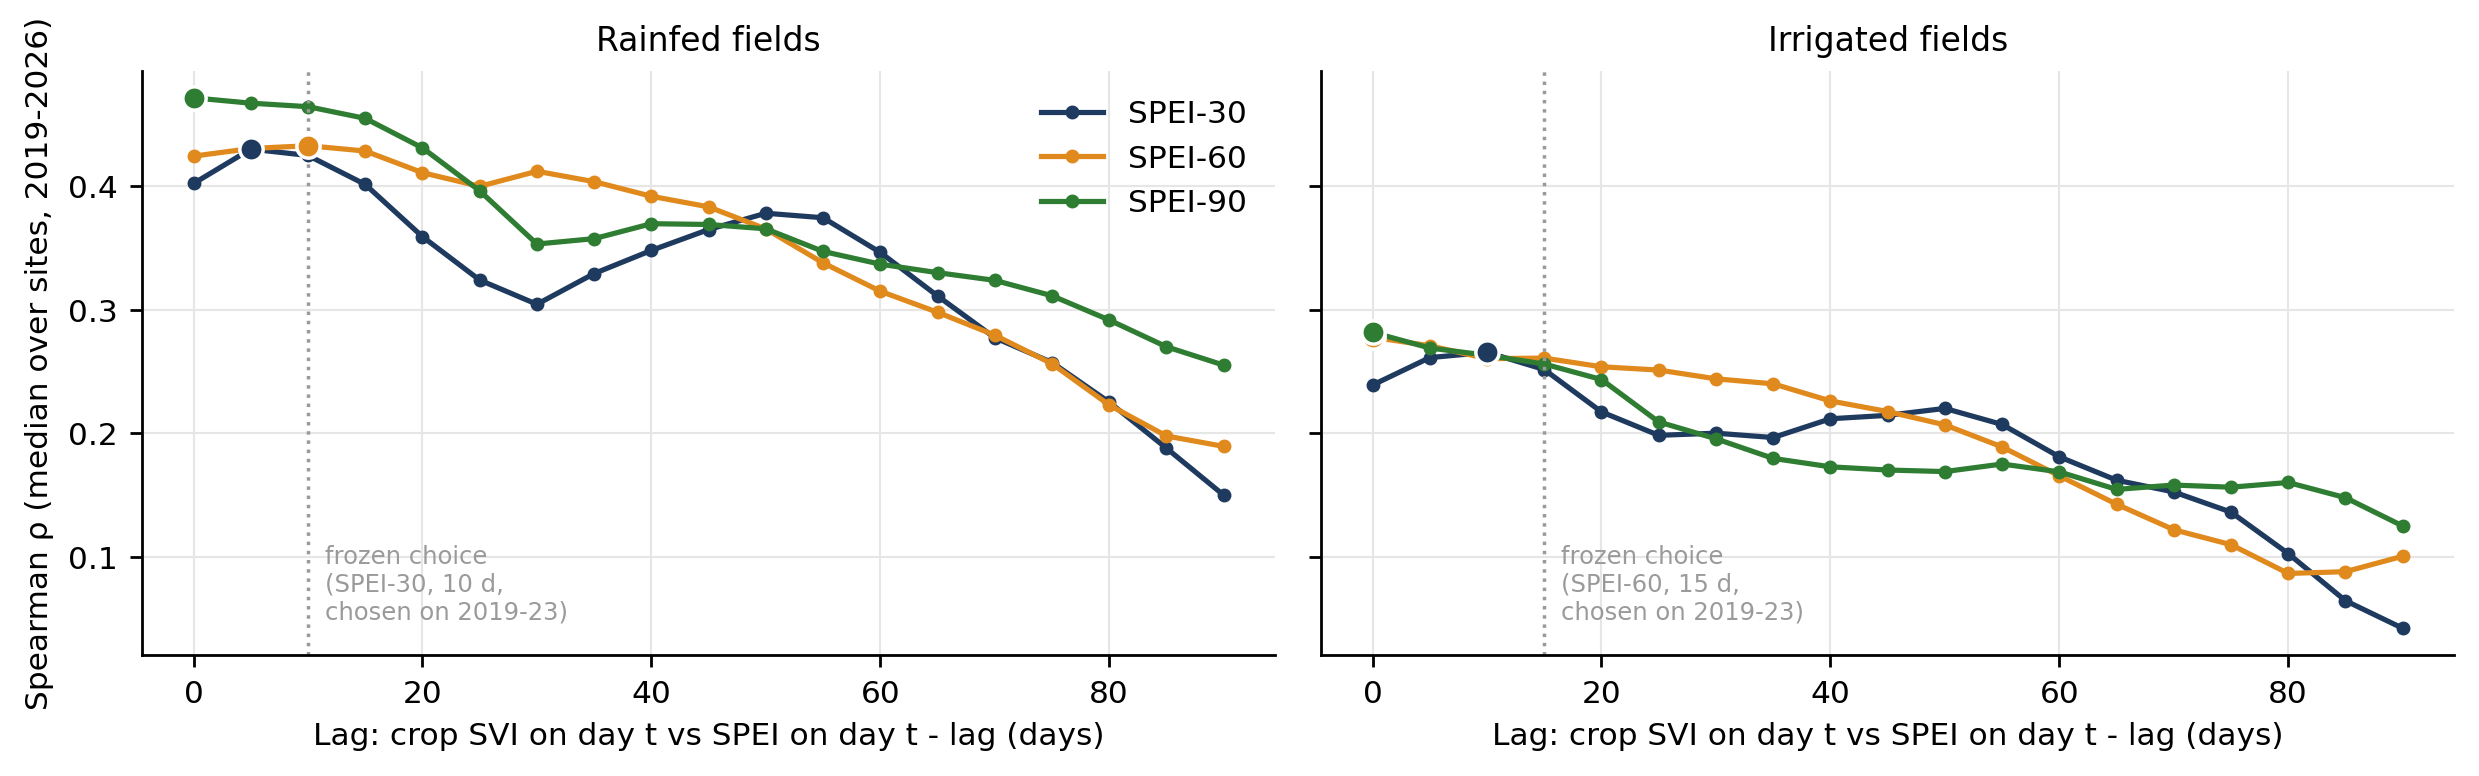
\includegraphics[width=0.97\textwidth]{figures/res_s_lag.png}
\caption{Correlation between crop SVI and lagged SPEI (median over sites, 2019--2026) for rainfed and irrigated fields. Dotted line: the frozen choice made on 2019--2023.}
\label{fig:s_lag}
\end{figure}

Weather alarms are followed by real crop stress far more often than chance (Table~\ref{tab:s_confirm}): in 22 of 44 alarms (50\,\%) rainfed crop stress followed within 60 days, against a base rate of 6--39\,\% of all dates being stressed. Confirmation is strongest at the Kurnool sites (Balaji Villas 86\,\%, Dinnedevarapadu 75\,\%) and weakest at Peddakadubur, whose deep black soils hold water longer.

% --- table s_confirm (generated by make_results.py)
\begin{table}[H]
\centering
\caption{Satellite module: weather alarms (SPEI-30 $< -1$, 2019--2026) followed by rainfed crop stress (SVI $< -1$) within 60 days, compared with the share of all dates that are stressed (base rate).}
\label{tab:s_confirm}
\footnotesize
\begin{tabular}{@{}lccccc@{}}
\toprule
\textbf{Site} & \textbf{Alarms} & \textbf{Confirmed} & \textbf{Rate} & \textbf{Base rate} & \textbf{Median delay (d)} \\
\midrule
Somandepalle & 5 & 1 & 20\,\% & 39\,\% & 55 \\
Lepakshi & 6 & 3 & 50\,\% & 34\,\% & 55 \\
Cholasamudram & 6 & 4 & 67\,\% & 38\,\% & 32 \\
Sira & 6 & 3 & 50\,\% & 29\,\% & 30 \\
Peddakadubur & 3 & 0 & 0\,\% & 6\,\% & -- \\
Kurnool-Dinnedevarapadu & 4 & 3 & 75\,\% & 36\,\% & 10 \\
Kurnool-Balaji Villas & 7 & 6 & 86\,\% & 29\,\% & 18 \\
Kurnool-Pullaiah & 7 & 2 & 29\,\% & 10\,\% & 8 \\
\textbf{All sites} & 44 & 22 & 50\,\% &  &  \\
\bottomrule
\end{tabular}
\end{table}


\subsubsection{Crop-condition forecasts and early warning of stress onset}
Table~\ref{tab:s_forecast} compares the four input versions with Random Forest and XGBoost. All versions beat persistence at 15 and 30 days. The most useful practical score is \emph{onset}: among fields that are normal today, the models rank those that will fall below normal by day 15 at ROC-AUC 0.76 (30 days: 0.69--0.72), against 0.72 / 0.65 for a logistic baseline on the current SVI and its trend. Persistence cannot predict onsets at all (AUC 0.50). Weather inputs help XGBoost slightly at 15 days, but against satellite history alone the gain is borderline and is not claimed. Weather alone is far weaker (0.40), confirming that crop condition must be observed, not inferred from weather.

% --- table s_forecast (generated by make_results.py)
\begin{table}[H]
\centering
\caption{Satellite module: crop-condition (SVI class) forecast on test years 2025--2026 (\mf, mean of 5 seeds) and onset warning (ROC-AUC for fields normal today that fall below normal by the target date).}
\label{tab:s_forecast}
\footnotesize
\resizebox{\textwidth}{!}{%
\begin{tabular}{@{}lcccccc@{}}
\toprule
\textbf{Version} & \textbf{RF 15 d} & \textbf{XGB 15 d} & \textbf{Onset AUC 15 d} & \textbf{RF 30 d} & \textbf{XGB 30 d} & \textbf{Onset AUC 30 d} \\
\midrule
Persistence & 0.648 & 0.648 & 0.50 & 0.520 & 0.520 & 0.50 \\
1\; Satellite history & 0.679 & 0.667 & 0.76 & 0.563 & 0.555 & 0.69 \\
2\; + past weather & 0.670 & 0.675 & 0.76 & 0.549 & 0.553 & 0.69 \\
3\; + weather-module forecast & 0.673 & 0.675 & 0.76 & 0.547 & 0.551 & 0.69 \\
4\; + actual future weather (upper bound) & 0.674 & 0.686 & 0.77 & 0.554 & 0.573 & 0.72 \\
Weather only & 0.433 & 0.404 & 0.58 & 0.436 & 0.364 & 0.51 \\
Logistic baseline on SVI level + trend &  &  & 0.72 &  &  & 0.65 \\
\bottomrule
\end{tabular}}
\end{table}


Table~\ref{tab:s_subsets} splits the 15-day test results. The models gain most where persistence is weakest: rainfed fields (+0.05), kharif targets (+0.05) and the 2026 drought season (+0.07 for Random Forest). In rabi months no version differs much from persistence, which motivated the separate rabi module (Section~7).

% --- table s_subsets (generated by make_results.py)
\begin{table}[H]
\centering
\caption{Satellite module: 15-day crop-condition forecast by field type and season (test 2025--2026, \mf; last column onset ROC-AUC of version 3).}
\label{tab:s_subsets}
\footnotesize
\resizebox{\textwidth}{!}{%
\begin{tabular}{@{}lcccccc@{}}
\toprule
\textbf{Subset} & \textbf{Persistence} & \textbf{Sat.\ RF} & \textbf{Sat.\ XGB} & \textbf{+ wx forecast XGB} & \textbf{Weather only} & \textbf{Onset AUC} \\
\midrule
All fields & 0.648 & 0.679 & 0.667 & 0.675 & 0.404 & 0.76 \\
Rainfed fields & 0.617 & 0.667 & 0.655 & 0.663 & 0.407 & 0.75 \\
Irrigated fields & 0.685 & 0.693 & 0.682 & 0.690 & 0.394 & 0.78 \\
Kharif targets (Jun--Nov) & 0.608 & 0.656 & 0.628 & 0.632 & 0.329 & 0.73 \\
Rabi targets (Dec--Mar) & 0.654 & 0.659 & 0.660 & 0.673 & 0.357 & 0.77 \\
2026 drought season (Jul--Nov) & 0.547 & 0.618 & 0.577 & 0.550 & 0.167 & 0.67 \\
\bottomrule
\end{tabular}}
\end{table}


\subsubsection{Operational replay against government declarations}
Table~\ref{tab:s_replay_sites} gives the outcome for every site and kharif season, and Table~\ref{tab:replay} summarises it. All 9 severe site-seasons were confirmed, 5 before the government order; in 2026 Balaji Villas and Dinnedevarapadu were confirmed 22 days before the order. The only false alarm is Dinnedevarapadu 2023, where 53\,\% of fields were in fact below normal but the mandal was not declared. The three moderate declarations of 2025 were all missed.

% --- table s_replay_sites (generated by make_results.py)
\begin{table}[H]
\centering
\caption{Operational replay per site and kharif season: official declaration and system result (``2 d before'' = confirmed 2 days before the government order). 2023 retrospective, 2024--2026 prospective; 2026 data to 24 October.}
\label{tab:s_replay_sites}
\footnotesize
\begin{tabular}{@{}lllll@{}}
\toprule
\textbf{Site} & \textbf{2023} & \textbf{2024} & \textbf{2025} & \textbf{2026} \\
\midrule
Somandepalle & Moderate: 2 d before & none: quiet & Moderate: missed & Severe: after order \\
Lepakshi & Moderate: 7 d before & none: quiet & Moderate: missed & Severe: 7 d before \\
Cholasamudram & Moderate: 12 d before & none: quiet & Moderate: missed & Severe: after order \\
Sira & Severe: 5 d before & no order found & no order found & likely declared: confirmed \\
Peddakadubur & ambiguous mandal & ambiguous mandal & none: quiet & ambiguous mandal \\
Kurnool-Dinnedevarapadu & none: \textit{false alarm} & none: quiet & none: quiet & Severe: 22 d before \\
Kurnool-Balaji Villas & Severe: 2 d before & none: quiet & none: quiet & Severe: 22 d before \\
Kurnool-Pullaiah & Severe: after order & none: quiet & none: quiet & Severe: after order \\
\bottomrule
\end{tabular}
\end{table}


\begin{table}[H]
\centering
\caption{Operational replay against official declarations (kharif 2023--2026). Each official decision is counted once at mandal level.}
\label{tab:replay}
\small
\begin{tabular}{@{}lcccc@{}}
\toprule
\multirow{2}{*}{\textbf{Official declaration}} & \multicolumn{2}{c}{\textbf{Site-seasons}} & \multicolumn{2}{c}{\textbf{Mandal-seasons}} \\
\cmidrule(lr){2-3}\cmidrule(lr){4-5}
 & \textbf{confirmed} & \textbf{before order} & \textbf{confirmed} & \textbf{before order} \\
\midrule
Severe & 9 / 9 & 5 / 9 & 6 / 6 & 5 / 6 \\
Moderate & 3 / 6 & 3 / 6 & 2 / 4 & 2 / 4 \\
Not declared (false alarm) & 1 / 11 & & 1 / 8 & \\
Prospective 2024--2026 only & severe 6/6 & severe 3/6 & false alarms 0/10 & \\
\bottomrule
\end{tabular}
\end{table}

Figure~\ref{fig:s_cases} shows how the system behaved in four seasons. At Balaji Villas (2023) and Dinnedevarapadu (2026) the weather alarm came first, crop SVI then fell below $-1$ and the system confirmed drought before the order. At Lepakshi (2026) confirmation came 7 days before the order. At Somandepalle (2025, declared moderate) rain was above normal and crops stayed greener than normal throughout June--November, so the system stayed silent: the declaration probably reflects late-season stress after the replay window.

\begin{figure}[H]
\centering
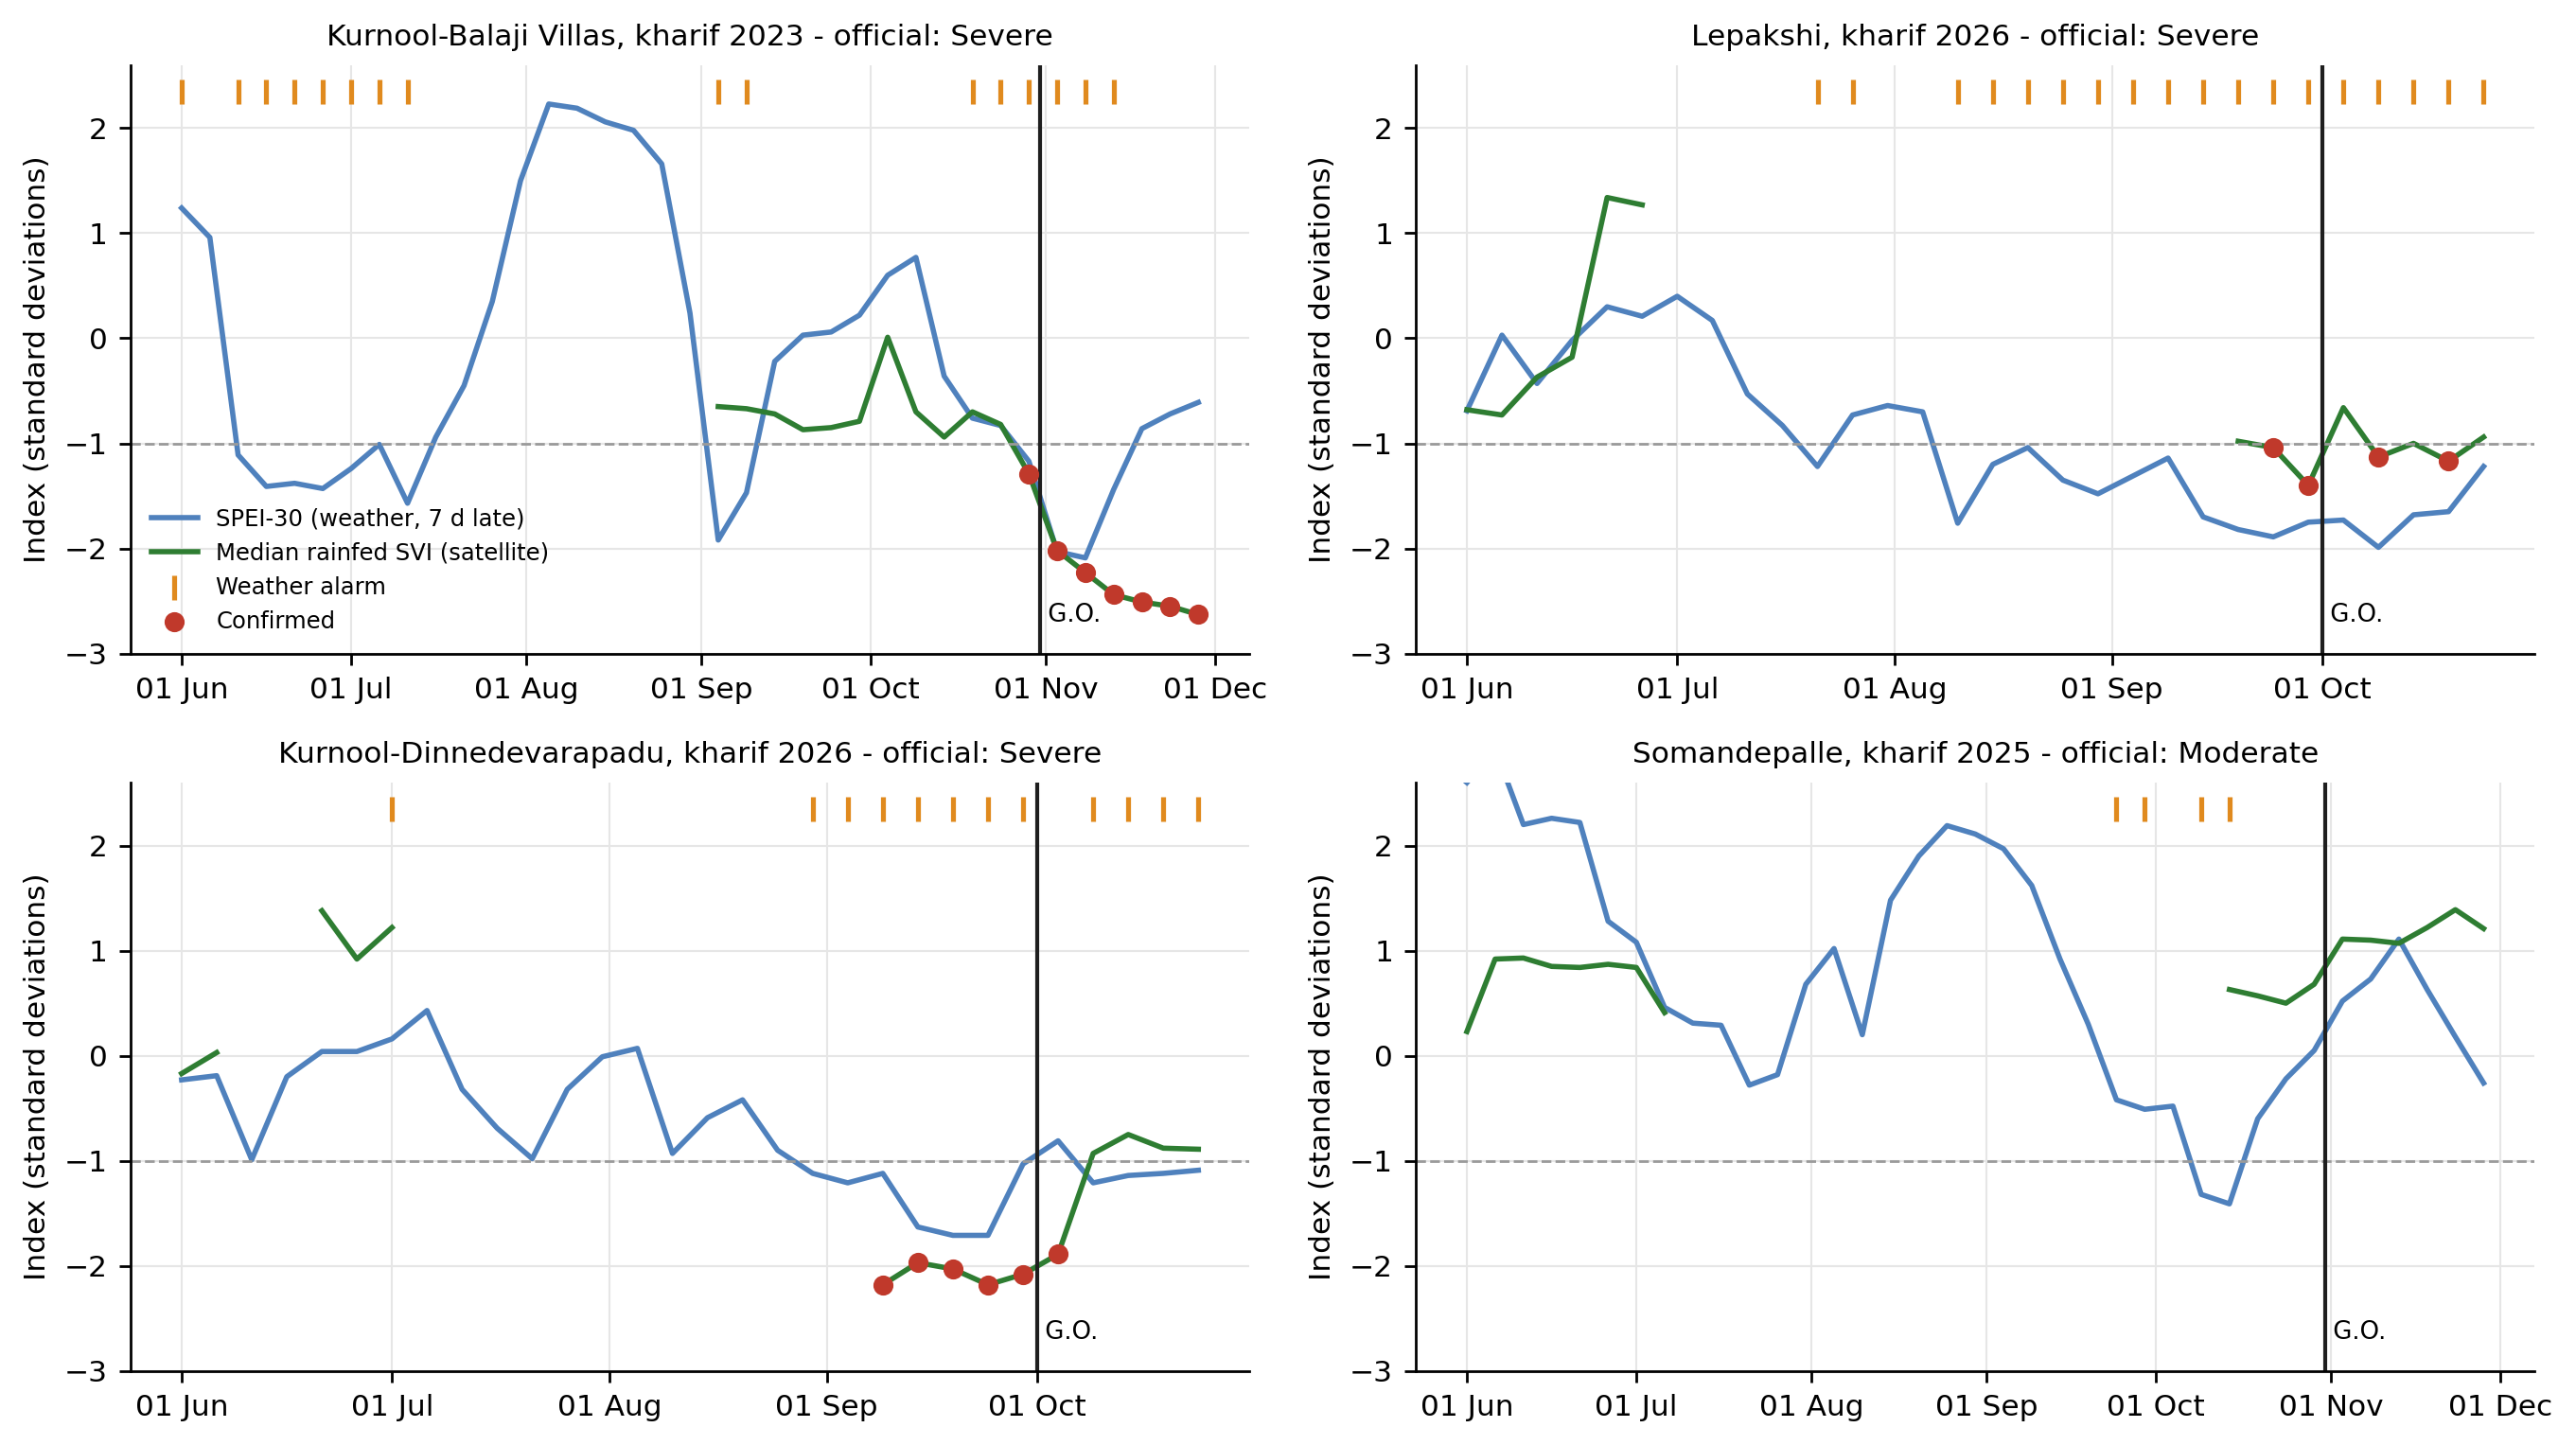
\includegraphics[width=\textwidth]{figures/res_s_cases.png}
\caption{Case studies from the operational replay: SPEI-30 available on each issue date (blue), median rainfed SVI (green), weather alarms (orange ticks), confirmed drought (red dots) and the government order date (G.O., black line).}
\label{fig:s_cases}
\end{figure}

% --- table s_seasons (generated by make_results.py)
\begin{table}[H]
\centering
\caption{Kharif season evidence per site: June--October rain vs normal, mean SPEI-30 and rainfed SVI in August--November, share of rainfed fields below normal, and the official order.}
\label{tab:s_seasons}
\scriptsize
\resizebox{\textwidth}{!}{%
\begin{tabular}{@{}llccccl@{}}
\toprule
\textbf{Year} & \textbf{Site} & \textbf{Rain} & \textbf{SPEI-30} & \textbf{SVI rainfed} & \textbf{Fields below normal} & \textbf{Official} \\
\midrule
2023 & Somandepalle & -36\,\% & -1.02 & -0.89 & 30\,\% & Moderate \\
 & Lepakshi & -31\,\% & -1.04 & -1.24 & 28\,\% & Moderate \\
 & Cholasamudram & -31\,\% & -1.04 & -1.46 & 24\,\% & Moderate \\
 & Sira & -23\,\% & -0.89 & -1.95 & 83\,\% & Severe \\
 & Peddakadubur & -10\,\% & -0.15 & -0.56 & 40\,\% & Moderate (Adoni) / Severe (Peddakadubur) \\
 & Kurnool-Dinnedevarapadu & -9\,\% & -0.09 & -1.57 & 53\,\% & Not declared \\
 & Kurnool-Balaji Villas & -6\,\% & +0.06 & -1.13 & 38\,\% & Severe \\
 & Kurnool-Pullaiah & -6\,\% & +0.06 & -0.19 & 30\,\% & Severe \\
\midrule
2025 & Somandepalle & +11\,\% & +0.47 & +0.82 & 0\,\% & Moderate \\
 & Lepakshi & +12\,\% & +0.50 & +0.32 & 6\,\% & Moderate \\
 & Cholasamudram & +12\,\% & +0.50 & +0.50 & 6\,\% & Moderate \\
 & Sira & +15\,\% & +0.50 & +0.12 & 0\,\% & Unknown \\
 & Peddakadubur & +37\,\% & +1.13 & +0.09 & 5\,\% & Not declared \\
 & Kurnool-Dinnedevarapadu & +39\,\% & +1.10 & +0.27 & 5\,\% & Not declared \\
 & Kurnool-Balaji Villas & +35\,\% & +0.99 & +0.25 & 10\,\% & Not declared \\
 & Kurnool-Pullaiah & +35\,\% & +0.99 & +0.04 & 5\,\% & Not declared \\
\midrule
2026 & Somandepalle & -52\,\% & -1.55 & -1.77 & 85\,\% & Severe \\
 & Lepakshi & -41\,\% & -1.38 & -1.22 & 56\,\% & Severe \\
 & Cholasamudram & -41\,\% & -1.38 & -1.40 & 59\,\% & Severe \\
 & Sira & -31\,\% & -1.26 & -1.59 & 70\,\% & Unknown (likely declared) \\
 & Peddakadubur & -57\,\% & -1.63 & -0.31 & 25\,\% & Severe (Adoni) / Not declared (Peddakadubur) \\
 & Kurnool-Dinnedevarapadu & -50\,\% & -1.27 & -1.27 & 68\,\% & Severe \\
 & Kurnool-Balaji Villas & -43\,\% & -1.06 & -1.03 & 33\,\% & Severe \\
 & Kurnool-Pullaiah & -43\,\% & -1.06 & -0.65 & 30\,\% & Severe \\
\bottomrule
\end{tabular}}
\end{table}


Table~\ref{tab:s_seasons} gives the physical evidence behind these outcomes. In 2026 June--October rain was 31--57\,\% below normal at all sites and most rainfed fields were below normal, except at Peddakadubur (driest, $-57$\,\%, but only a quarter of fields below normal). In 2025 rain was above normal, explaining the missed moderate declarations.

\subsubsection{Comparison with UAV fields}
At the 10 UAV survey fields (Table~\ref{tab:s_uav}) satellite and drone verdicts agree clearly at 3 fields and partly at 2. Most flights were made after harvest (November 2025 -- January 2026), when Sentinel-2 measures residue or regrowth, and a field with 40\,\% dry patches can still look normal in a 10\,m pixel. This is the reason for the UAV stage: the satellite says \emph{where}, the drone measures \emph{how much}.

% --- table s_uav (generated by make_results.py)
\begin{table}[H]
\centering
\caption{UAV field verdicts vs the Sentinel-2 verdict at the flight date.}
\label{tab:s_uav}
\footnotesize
\begin{tabular}{@{}lllll@{}}
\toprule
\textbf{UAV field} & \textbf{Crop} & \textbf{UAV verdict} & \textbf{Satellite verdict} & \textbf{SVI} \\
\midrule
Peddakadubur & Cotton & mixed & not stressed & +0.75 \\
Dinnedevarapadu & Cotton & healthy & not stressed & +0.54 \\
Balaji Villas & Cotton & healthy & stressed & +0.82 \\
Shilpa Township & Cotton & healthy & not stressed & +0.61 \\
Puddur & Maize & healthy & not stressed & +1.27 \\
Pullaiah College & Cotton & healthy & stressed & -1.02 \\
Cholasamudram & Maize & drought & not stressed & +0.04 \\
Lepakshi & Maize & drought & not stressed & -0.77 \\
Somandepalli & Maize & drought & not stressed & +1.38 \\
Sira & Cotton+Maize & drought  / healthy & not stressed & -0.18 \\
\bottomrule
\end{tabular}
\end{table}


Applied to rabi (December--March), the same chain confirmed none of the 4 severe rabi mandal-seasons on in-season images, which motivated the separate rabi module.

% ============================================================================
\section{Module 2b: Rabi Vegetation Forecast}

\subsection{Why a separate rabi method}
Rabi crops grow on stored soil water and irrigation rather than current rain and often fail late (terminal drought~\cite{pang2017}); early-season drought is hard to see with conventional indices~\cite{nikam2020}. There are also too few rabi declarations to train a classifier. The rabi module therefore forecasts \textbf{crop greenness}, whose target comes from future satellite images rather than government orders. Earlier rule-based attempts on 233 historically rabi-active fields (protocol v1) flagged none of the 4 severe rabi mandal-seasons in a development check; the selected fields were biased toward resilient fields, which led to random whole-mandal sampling.

\subsection{Method}
All rules were written and committed to git \emph{before} any model was trained; two independent reviews led to documented amendments (climatology at issue date + 15 days, frozen-calibration weather, 8-day weather delay, training-only fallback normals). The final version is frozen as tag \texttt{rabi-forecast-v1-final}.

\textbf{Points.} In 9 mandals (2018 LGD polygons: Somandepalle, Lepakshi, Chilamathur, Sira, Agali, Adoni, Pedda Kadubur, Kurnool, Kallur), cropland is WorldCover 2020 \emph{and} 2021 cropland; irrigated = March--May NDVI 75th percentile $> 0.4$ in at least 2 of the summers 2019--2023. A stratified random sample gives 100 rainfed + 50 irrigated points per mandal = \textbf{1,350 points}. For each, mean NDVI in a 15\,m buffer is extracted from every clear Sentinel-2 image, October--April 2019-20 to 2025-26 (355,043 rows; 313,797 after cleaning: $\ge 12$ of $\sim$16 pixels clear, NDVI in $[-0.2, 1]$, one observation per point and date).

\textbf{Forecast instances} (Fig.~\ref{fig:rabi_rules}). A forecast is issued every 5 days at date $t$. It is used only if the latest image dated $\le t-2$ days is at most 12 days old, and a real image exists at $t+15 \pm 3$ days (no interpolation). Excluded forecasts are missing data, never ``no crop''.

\textbf{Inputs and model.} NDVI now, 15 and 30 days ago, changes, ages, season minimum and maximum, observation count, day of season, rainfed/irrigated, location; the point's training-season normal at $t+15$ and at the latest observation; AgERA5 weather available 8 days late (rain over 30 / 90 days, rain since June vs normal, ET$_0$, $T_{\max}$, 60-day water balance, frozen SPEI). XGBoost regresses the 15-day change; the forecast is
\begin{equation}
\widehat{\mathrm{NDVI}}_{t+15} = \mathrm{NDVI}_{\text{last}} + f_{\text{XGB}}(\mathbf{x}_t).
\end{equation}
Baselines: persistence ($\mathrm{NDVI}_{\text{last}}$), climatology (point normal at $t+15$) and anomaly persistence (normal at $t+15$ + today's anomaly). Split: train 2019-20 -- 2021-22, validation 2022-23 (early stopping), refit 2019-20 -- 2022-23, \textbf{test 2023-24, 2024-25, 2025-26}. Metric: mean absolute error (MAE) of NDVI. Pre-registered acceptance rule: lower MAE than every baseline in each test season and a 95\,\% bootstrap interval of the pooled MAE difference entirely below 0.

\begin{figure}[H]
\centering
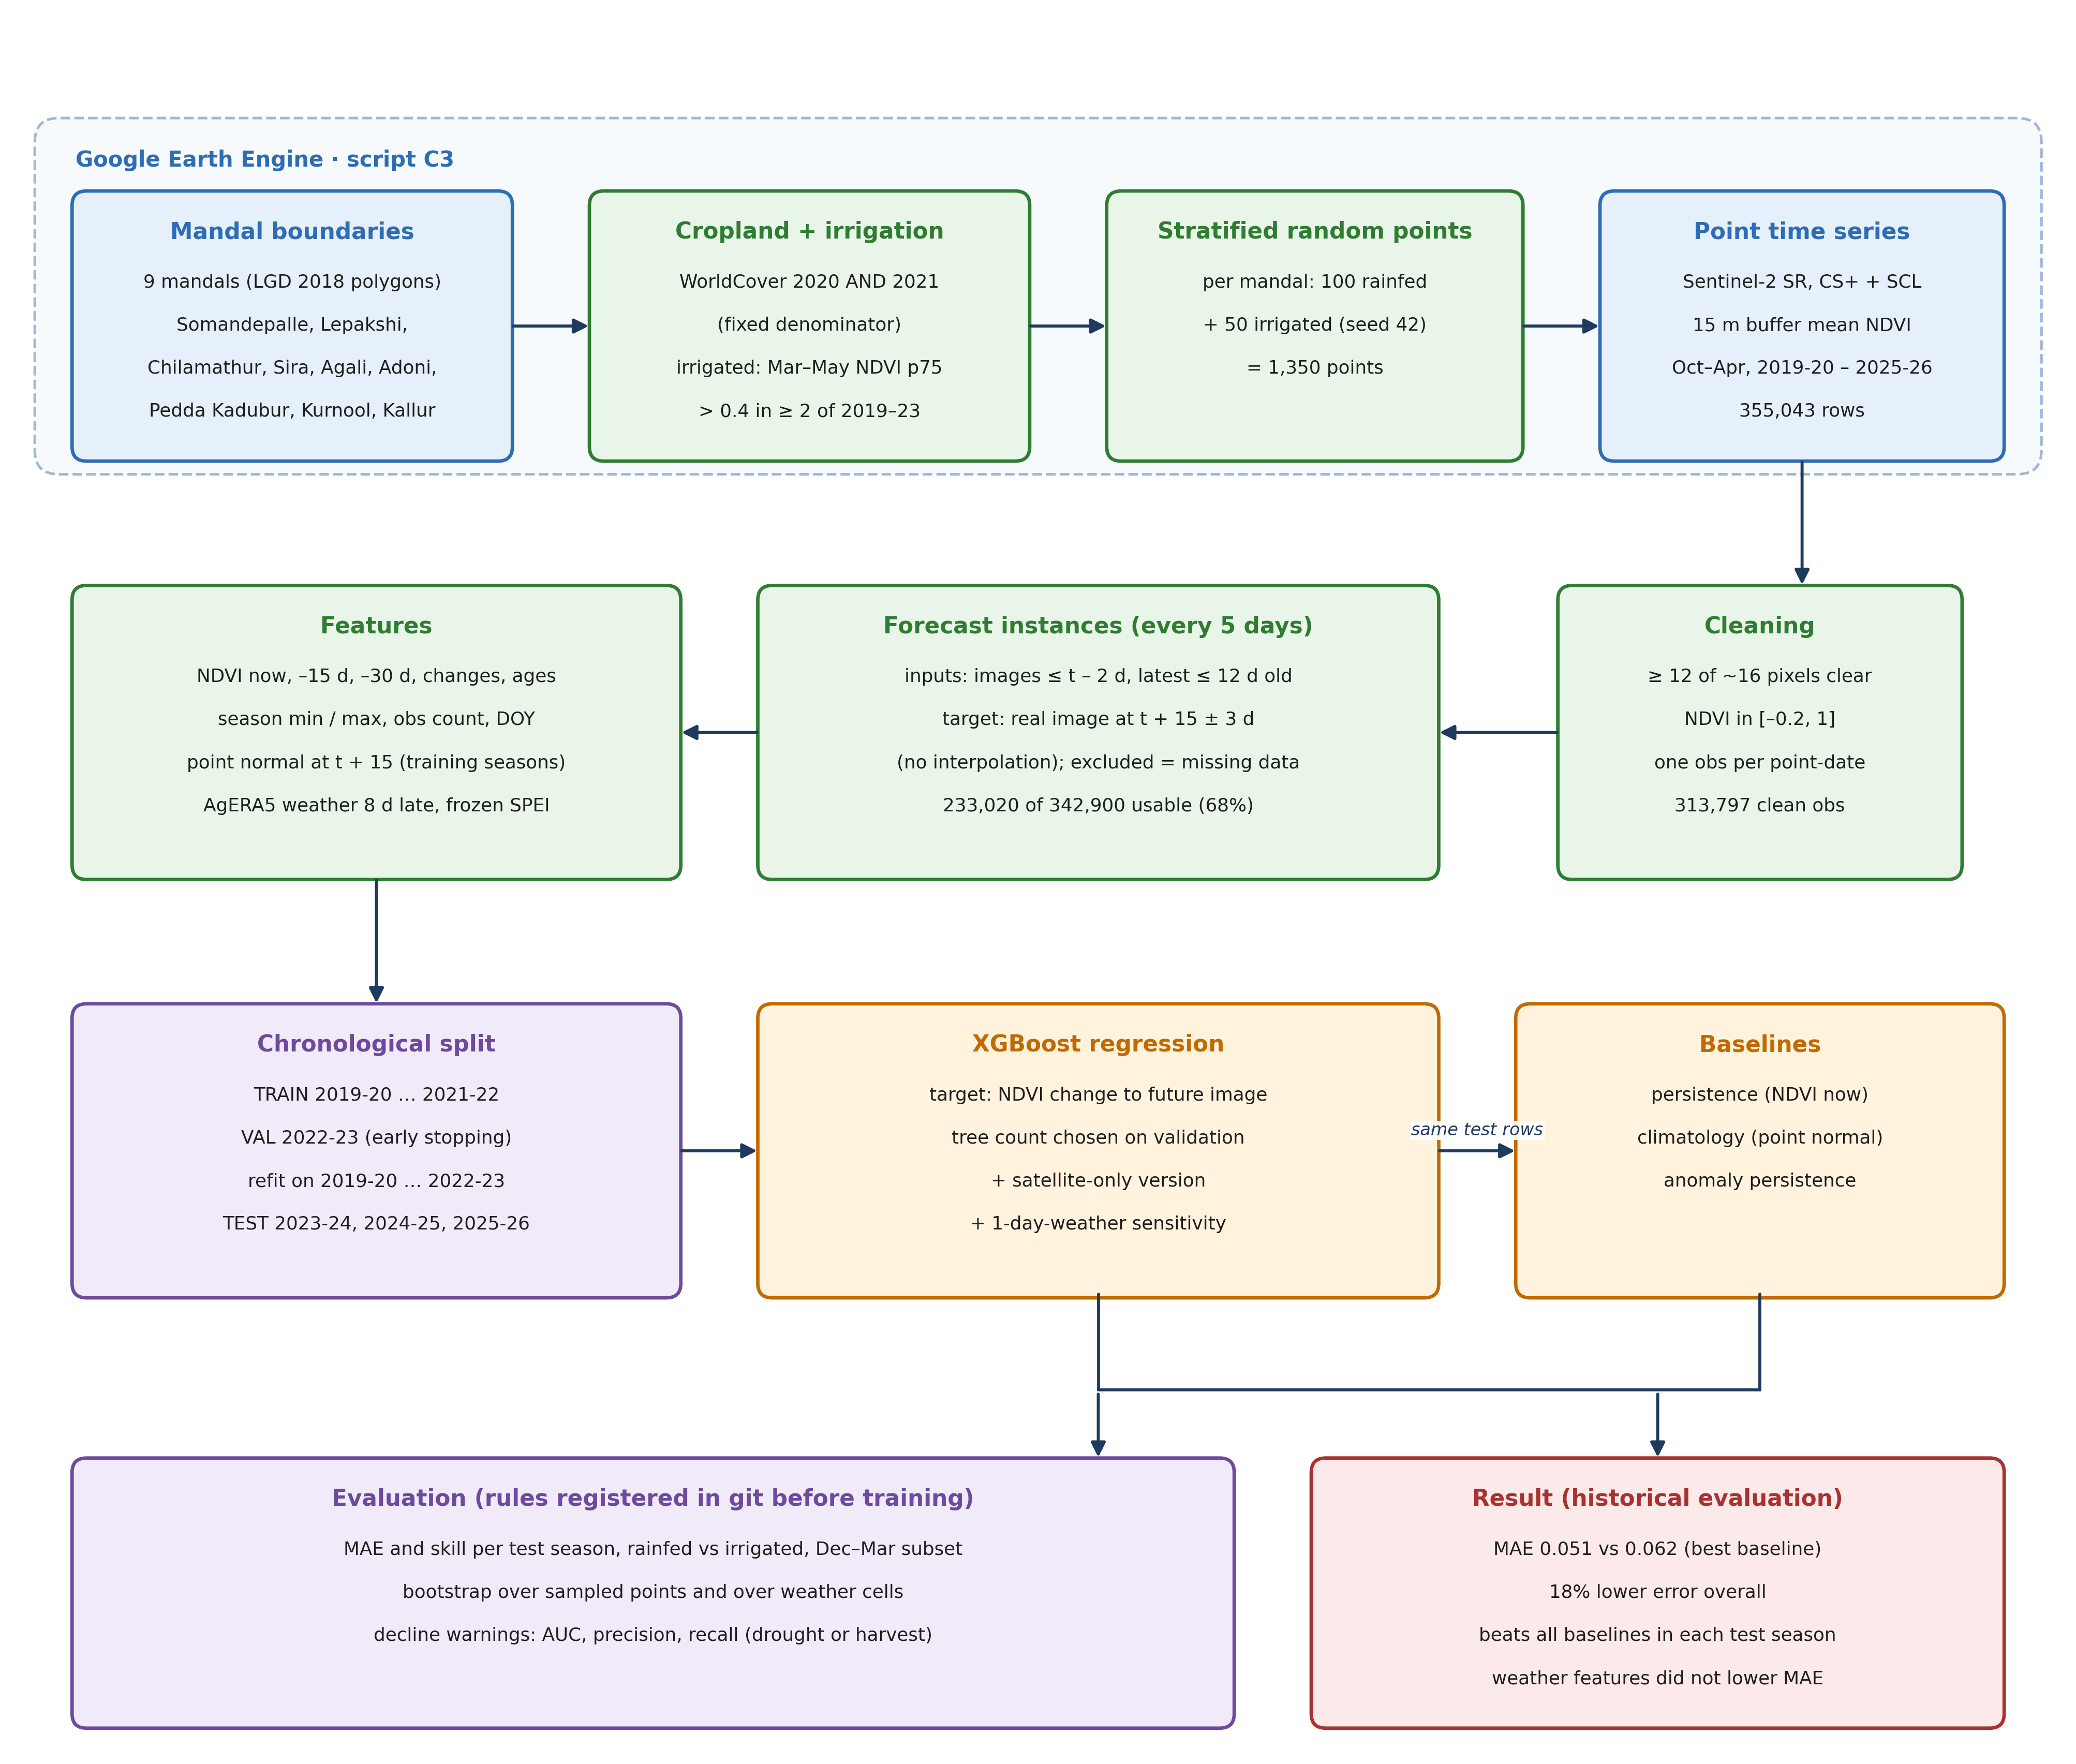
\includegraphics[width=0.95\textwidth]{figures/fig4_rabi_module_architecture.png}
\caption{Rabi module architecture (15-day vegetation forecast).}
\label{fig:rabi_arch}
\end{figure}

\begin{figure}[H]
\centering
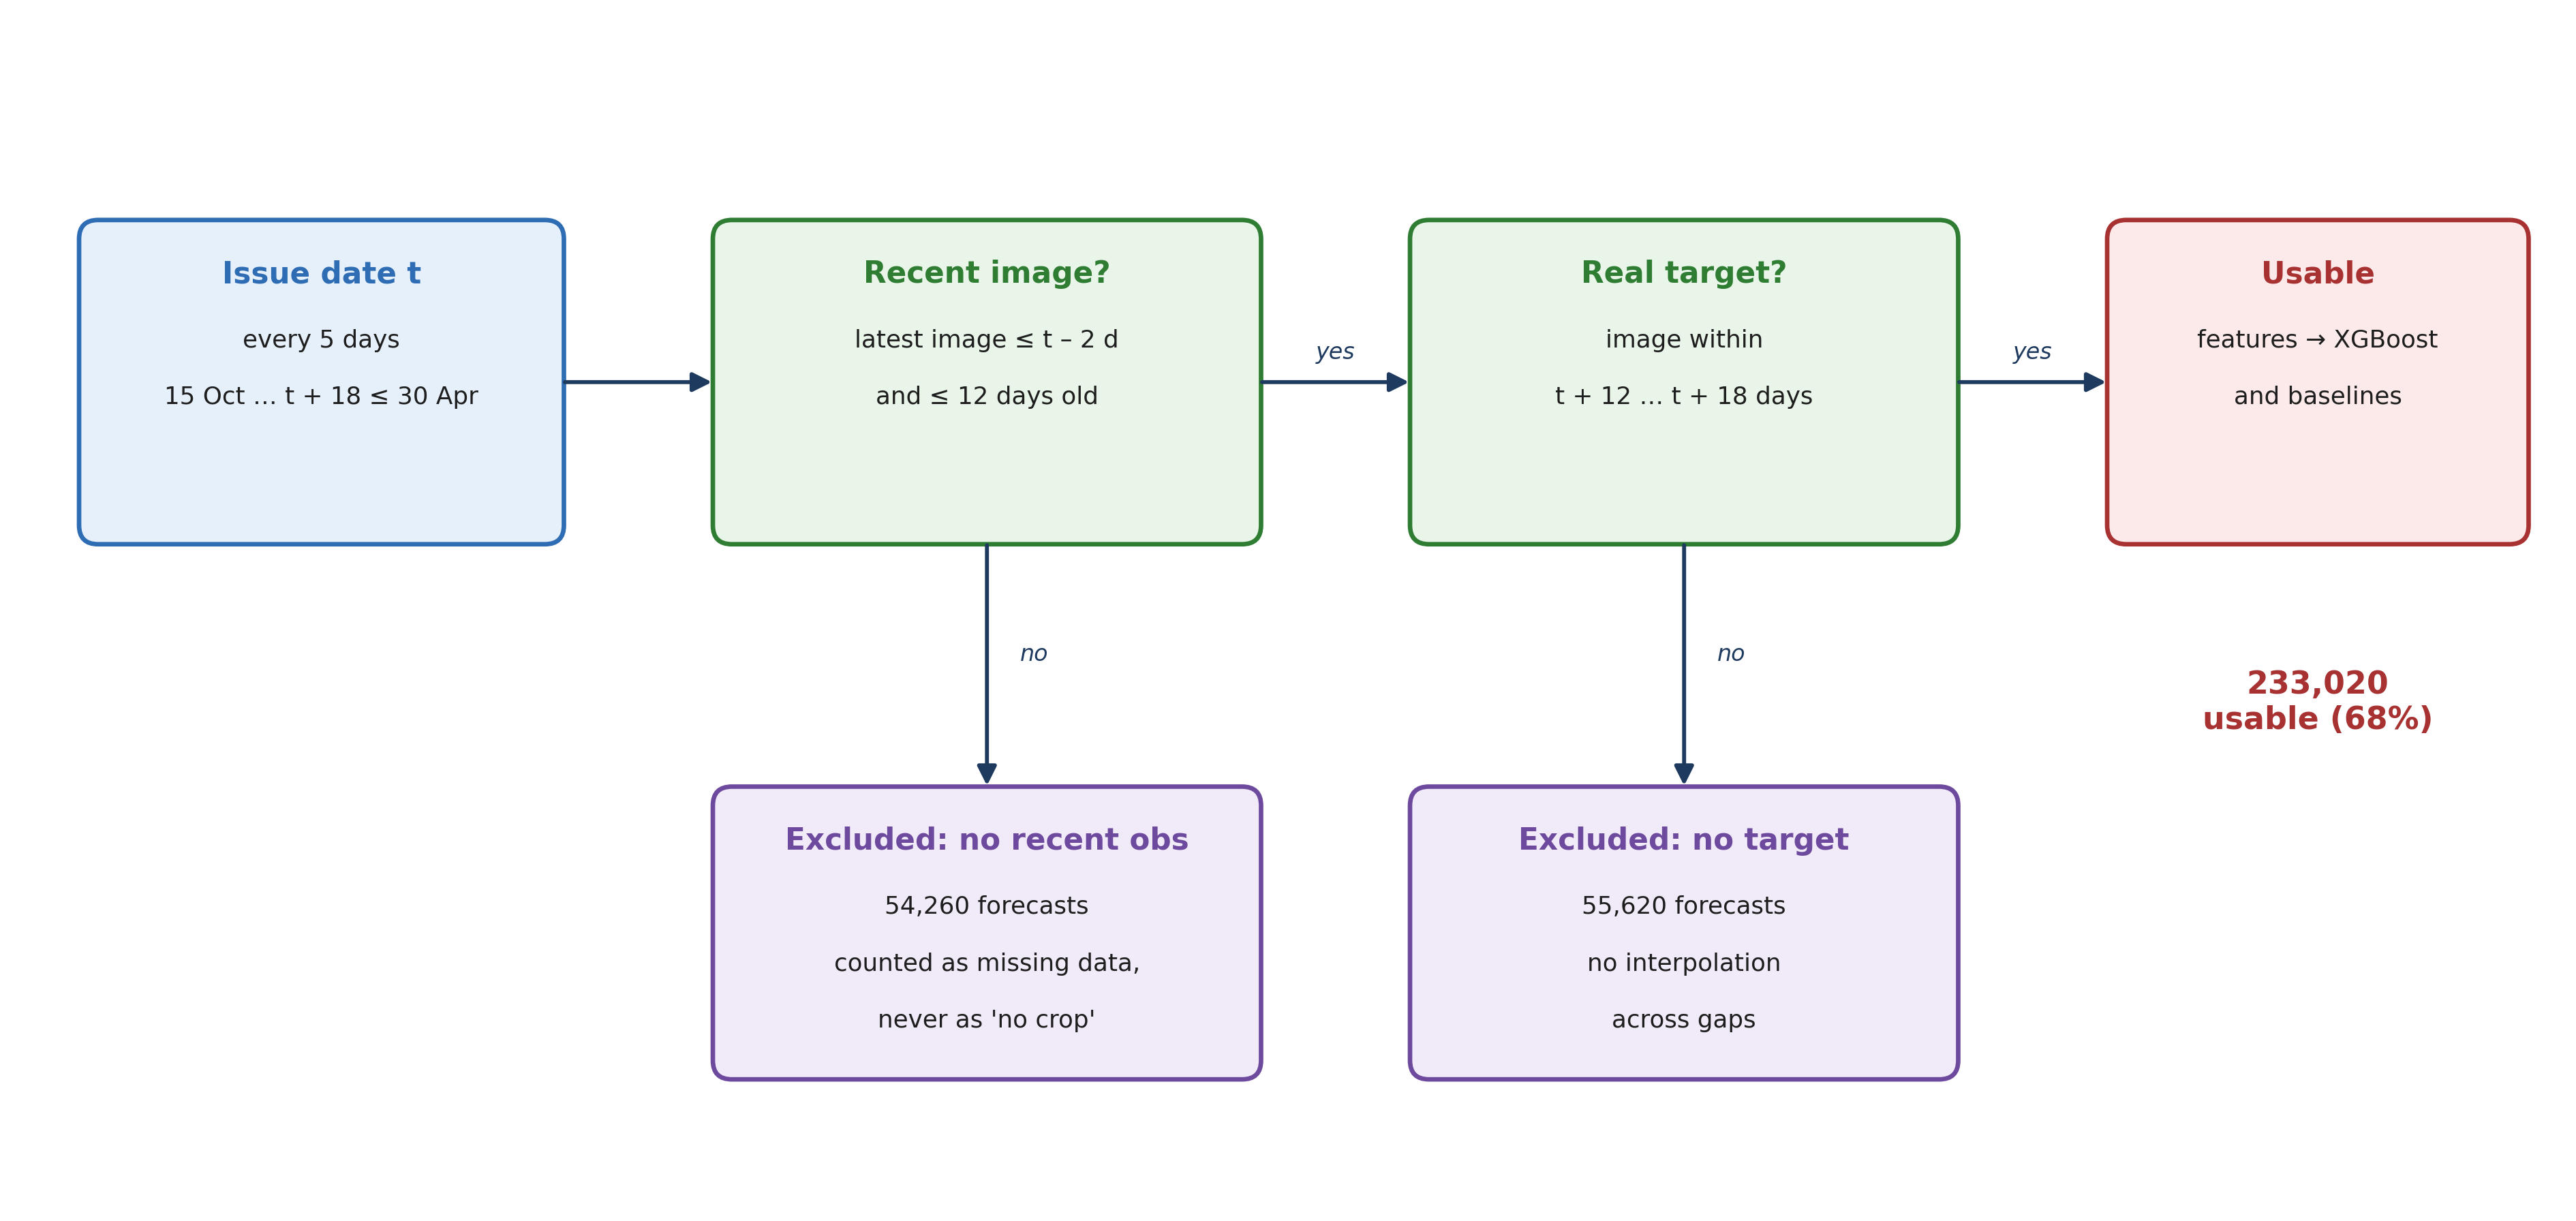
\includegraphics[width=0.85\textwidth]{figures/fig7_rabi_forecast_rules.png}
\caption{Eligibility and target rules of one rabi forecast: 233,020 of 342,900 potential forecasts (68\,\%) are usable.}
\label{fig:rabi_rules}
\end{figure}

\subsection{Results}

\subsubsection{Development of the rabi method}
Table~\ref{tab:r_history} summarises how the rabi method was developed. Applying the kharif chain or rule-based establishment checks on historically rabi-active fields did not identify the declared rabi droughts. An exploratory early-drying signal caught 2 of 4, but it was designed after seeing those seasons. Measuring the whole mandal instead of selected fields shows the 2023-24 dry season clearly (Table~\ref{tab:r_c3}): the irrigated area established by March fell to 17\,\% at Adoni (normal 44\,\%) and 28\,\% at Pedda Kadubur (normal 48\,\%). This led to the final design: random whole-mandal points and a forecast of greenness rather than a classifier of declarations.

% --- table r_history (generated by make_results.py)
\begin{table}[H]
\centering
\caption{Development of the rabi method: severe rabi mandal-seasons flagged and undeclared mandal-seasons flagged (2023-24 to 2025-26).}
\label{tab:r_history}
\footnotesize
\begin{tabular}{@{}lccl@{}}
\toprule
\textbf{Approach} & \textbf{Severe flagged} & \textbf{Undeclared flagged} & \textbf{Note} \\
\midrule
Kharif chain applied to rabi (replay) & 0 / 4 & 0 / 10 & in-season images only \\
Protocol v1 on 233 rabi-candidate fields & 0 / 4 & 5 / 10 & development check 2023--26 \\
Early-drying signal (exploratory) & 2 / 4 & 1 / 10 & post hoc, retrospective \\
Whole-mandal 15-day NDVI forecast (final) & \multicolumn{2}{c}{forecasts greenness, not drought} & 18\,\% lower error, all test seasons \\
\bottomrule
\end{tabular}
\end{table}

% --- table r_c3 (generated by make_results.py)
\begin{table}[H]
\centering
\caption{Exploratory: share (\%) of irrigated cropland in each mandal that turned green (established) by March, per rabi season, from the whole-mandal Sentinel-2 summary. Bold = below 75\,\% of the 2019--2022 normal. Seasons were known during design.}
\label{tab:r_c3}
\footnotesize
\begin{tabular}{@{}lcccccccc@{}}
\toprule
\textbf{Mandal} & \textbf{19-20} & \textbf{20-21} & \textbf{21-22} & \textbf{22-23} & \textbf{23-24} & \textbf{24-25} & \textbf{25-26} & \textbf{Normal} \\
\midrule
Somandepalle & 30 & 35 & 25 & 34 & \textbf{23} & 32 & 27 & 31 \\
Lepakshi & 14 & 22 & 21 & 29 & 25 & 22 & 26 & 21 \\
Chilamathur & 18 & 26 & 26 & 35 & 24 & 27 & 27 & 26 \\
Sira & 12 & 13 & 14 & 20 & 13 & 13 & 12 & 15 \\
Agali & 12 & 18 & 18 & 28 & 21 & 16 & 19 & 19 \\
Adoni & 36 & 49 & 40 & 51 & \textbf{17} & 50 & \textbf{24} & 44 \\
Pedda Kadubur & 45 & 47 & 37 & 64 & \textbf{28} & 52 & 55 & 48 \\
Kurnool & 44 & 55 & 52 & 59 & 43 & 49 & 52 & 52 \\
Kallur & 38 & 49 & 49 & 51 & 47 & 44 & 49 & 47 \\
\bottomrule
\end{tabular}
\end{table}


\subsubsection{Forecast accuracy}
% --- table r_eligibility (generated by make_results.py)
\begin{table}[H]
\centering
\caption{Rabi forecast eligibility per season: potential forecasts, exclusions (missing data, never ``no crop'') and usable forecasts.}
\label{tab:r_elig}
\footnotesize
\begin{tabular}{@{}lrrrrr@{}}
\toprule
\textbf{Season} & \textbf{Potential} & \textbf{No recent image} & \textbf{No target image} & \textbf{Usable} & \textbf{Share} \\
\midrule
2019-20 & 49,950 & 9,947 & 9,947 & 30,056 & 60\,\% \\
2020-21 & 48,600 & 8,438 & 8,862 & 31,300 & 64\,\% \\
2021-22 & 48,600 & 8,836 & 9,282 & 30,482 & 63\,\% \\
2022-23 & 48,600 & 5,538 & 7,474 & 35,588 & 73\,\% \\
2023-24 & 49,950 & 5,652 & 8,790 & 35,508 & 71\,\% \\
2024-25 & 48,600 & 9,306 & 6,414 & 32,880 & 68\,\% \\
2025-26 & 48,600 & 6,543 & 4,851 & 37,206 & 77\,\% \\
\textbf{All} & 342,900 & 54,260 & 55,620 & 233,020 & 68\,\% \\
\bottomrule
\end{tabular}
\end{table}


Table~\ref{tab:r_elig} shows how many forecasts each season could be scored: 60--77\,\% depending on cloud cover, with 2025-26 the clearest season. Table~\ref{tab:rabi} gives the main result, and Table~\ref{tab:r_breakdown} breaks it down. XGBoost has the lowest error in every season, for both rainfed and irrigated land, and for both all points and crops already established. The gain is largest on rainfed land (about 19\,\%) and smallest on irrigated land in the dry season 2023-24 (9\,\%), where persistence is already a good guess.

\begin{table}[H]
\centering
\caption{Rabi 15-day NDVI forecast: MAE on held-out seasons (lower is better).}
\label{tab:rabi}
\small
\begin{tabular}{@{}lccc@{}}
\toprule
\textbf{Held-out season} & \textbf{XGBoost} & \textbf{Best baseline} & \textbf{Lower error} \\
\midrule
2023-24 & 0.046 & 0.054 (persistence) & 14\,\% \\
2024-25 & 0.051 & 0.061 (anomaly persistence) & 16\,\% \\
2025-26 & 0.056 & 0.068 (anomaly persistence) & 17\,\% \\
\textbf{All three} & \textbf{0.051} & \textbf{0.062} (anomaly persistence) & \textbf{18\,\%} \\
\bottomrule
\end{tabular}
\end{table}

% --- table r_breakdown (generated by make_results.py)
\begin{table}[H]
\centering
\caption{Rabi forecast by test season, field type and population (MAE of NDVI 15 days ahead).}
\label{tab:r_breakdown}
\scriptsize
\begin{tabular}{@{}lllrcccr@{}}
\toprule
\textbf{Population} & \textbf{Season} & \textbf{Class} & \textbf{Forecasts} & \textbf{XGBoost} & \textbf{Best baseline} & \textbf{Which baseline} & \textbf{Lower error} \\
\midrule
All eligible points & 2023-24 & rainfed & 23,722 & 0.0371 & 0.0452 & Persistence & 18\,\% \\
 &  & irrigated & 11,786 & 0.0639 & 0.0702 & Persistence & 9\,\% \\
 &  & all & 35,508 & 0.0460 & 0.0535 & Persistence & 14\,\% \\
 & 2024-25 & rainfed & 21,872 & 0.0407 & 0.0498 & Anomaly persistence & 18\,\% \\
 &  & irrigated & 11,008 & 0.0722 & 0.0828 & Anomaly persistence & 13\,\% \\
 &  & all & 32,880 & 0.0512 & 0.0608 & Anomaly persistence & 16\,\% \\
 & 2025-26 & rainfed & 24,825 & 0.0464 & 0.0568 & Anomaly persistence & 18\,\% \\
 &  & irrigated & 12,381 & 0.0750 & 0.0878 & Persistence & 15\,\% \\
 &  & all & 37,206 & 0.0559 & 0.0675 & Anomaly persistence & 17\,\% \\
 & pooled & rainfed & 70,419 & 0.0415 & 0.0512 & Anomaly persistence & 19\,\% \\
 &  & irrigated & 35,175 & 0.0704 & 0.0814 & Persistence & 14\,\% \\
 &  & all & 105,594 & 0.0511 & 0.0623 & Anomaly persistence & 18\,\% \\
\midrule
Established at issue & 2023-24 & rainfed & 17,544 & 0.0331 & 0.0424 & Persistence & 22\,\% \\
 &  & irrigated & 9,940 & 0.0629 & 0.0697 & Persistence & 10\,\% \\
 &  & all & 27,484 & 0.0439 & 0.0523 & Persistence & 16\,\% \\
 & 2024-25 & rainfed & 18,303 & 0.0380 & 0.0463 & Anomaly persistence & 18\,\% \\
 &  & irrigated & 9,446 & 0.0714 & 0.0822 & Anomaly persistence & 13\,\% \\
 &  & all & 27,749 & 0.0494 & 0.0585 & Anomaly persistence & 16\,\% \\
 & 2025-26 & rainfed & 20,524 & 0.0427 & 0.0520 & Anomaly persistence & 18\,\% \\
 &  & irrigated & 10,699 & 0.0729 & 0.0846 & Persistence & 14\,\% \\
 &  & all & 31,223 & 0.0531 & 0.0637 & Anomaly persistence & 17\,\% \\
 & pooled & rainfed & 56,371 & 0.0382 & 0.0473 & Anomaly persistence & 19\,\% \\
 &  & irrigated & 30,085 & 0.0691 & 0.0801 & Persistence & 14\,\% \\
 &  & all & 86,456 & 0.0490 & 0.0597 & Anomaly persistence & 18\,\% \\
\bottomrule
\end{tabular}
\end{table}


XGBoost forecast NDVI approximately 15 days ahead with about 18\,\% lower mean absolute error overall than the best simple baseline. It outperformed all three baselines in each held-out season, with seasonal improvements of 14--17\,\%, and passed the pre-registered acceptance rule (95\,\% interval of the error difference, resampling sampled points: $[-0.012, -0.010]$; resampling the 5 weather cells: $[-0.015, -0.008]$). The advantage holds when only December--March issue dates are scored (Table~\ref{tab:r_decmar}), so it is not limited to the October--November sowing period.

% --- table r_decmar (generated by make_results.py)
\begin{table}[H]
\centering
\caption{Rabi forecast, December--March issue dates only.}
\label{tab:r_decmar}
\footnotesize
\begin{tabular}{@{}lrccr@{}}
\toprule
\textbf{Season} & \textbf{Forecasts} & \textbf{XGBoost} & \textbf{Best baseline} & \textbf{Lower error} \\
\midrule
2023-24 & 26,790 & 0.0412 & 0.0520 & 21\,\% \\
2024-25 & 25,687 & 0.0481 & 0.0569 & 15\,\% \\
2025-26 & 29,356 & 0.0521 & 0.0617 & 16\,\% \\
pooled & 81,833 & 0.0473 & 0.0570 & 17\,\% \\
\bottomrule
\end{tabular}
\end{table}


Figure~\ref{fig:r_month} shows the error by month. All methods are least accurate in October--December, when fields are being sown and NDVI changes fast; XGBoost gains most exactly there (e.g.\ November: 0.073 vs 0.090 for persistence) and stays best until April. Figure~\ref{fig:r_scatter} compares predicted and observed 15-day changes: the correlation rises from 0.27 for the best baseline to 0.54 for XGBoost, although large drops are still under-predicted.

\begin{figure}[H]
\centering
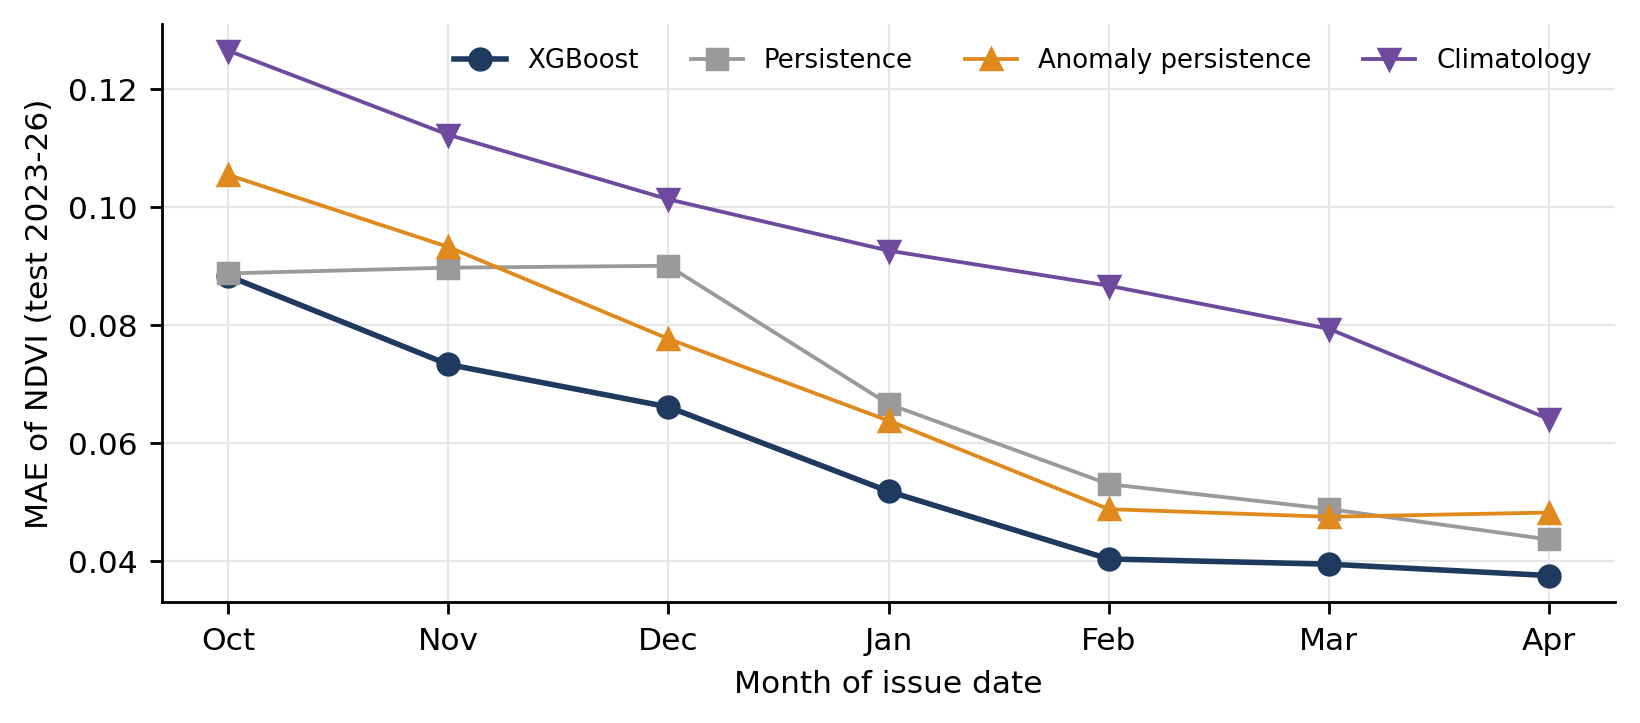
\includegraphics[width=0.82\textwidth]{figures/res_r_month.png}
\caption{Rabi forecast error by month of issue (test 2023-24 to 2025-26).}
\label{fig:r_month}
\end{figure}

\begin{figure}[H]
\centering
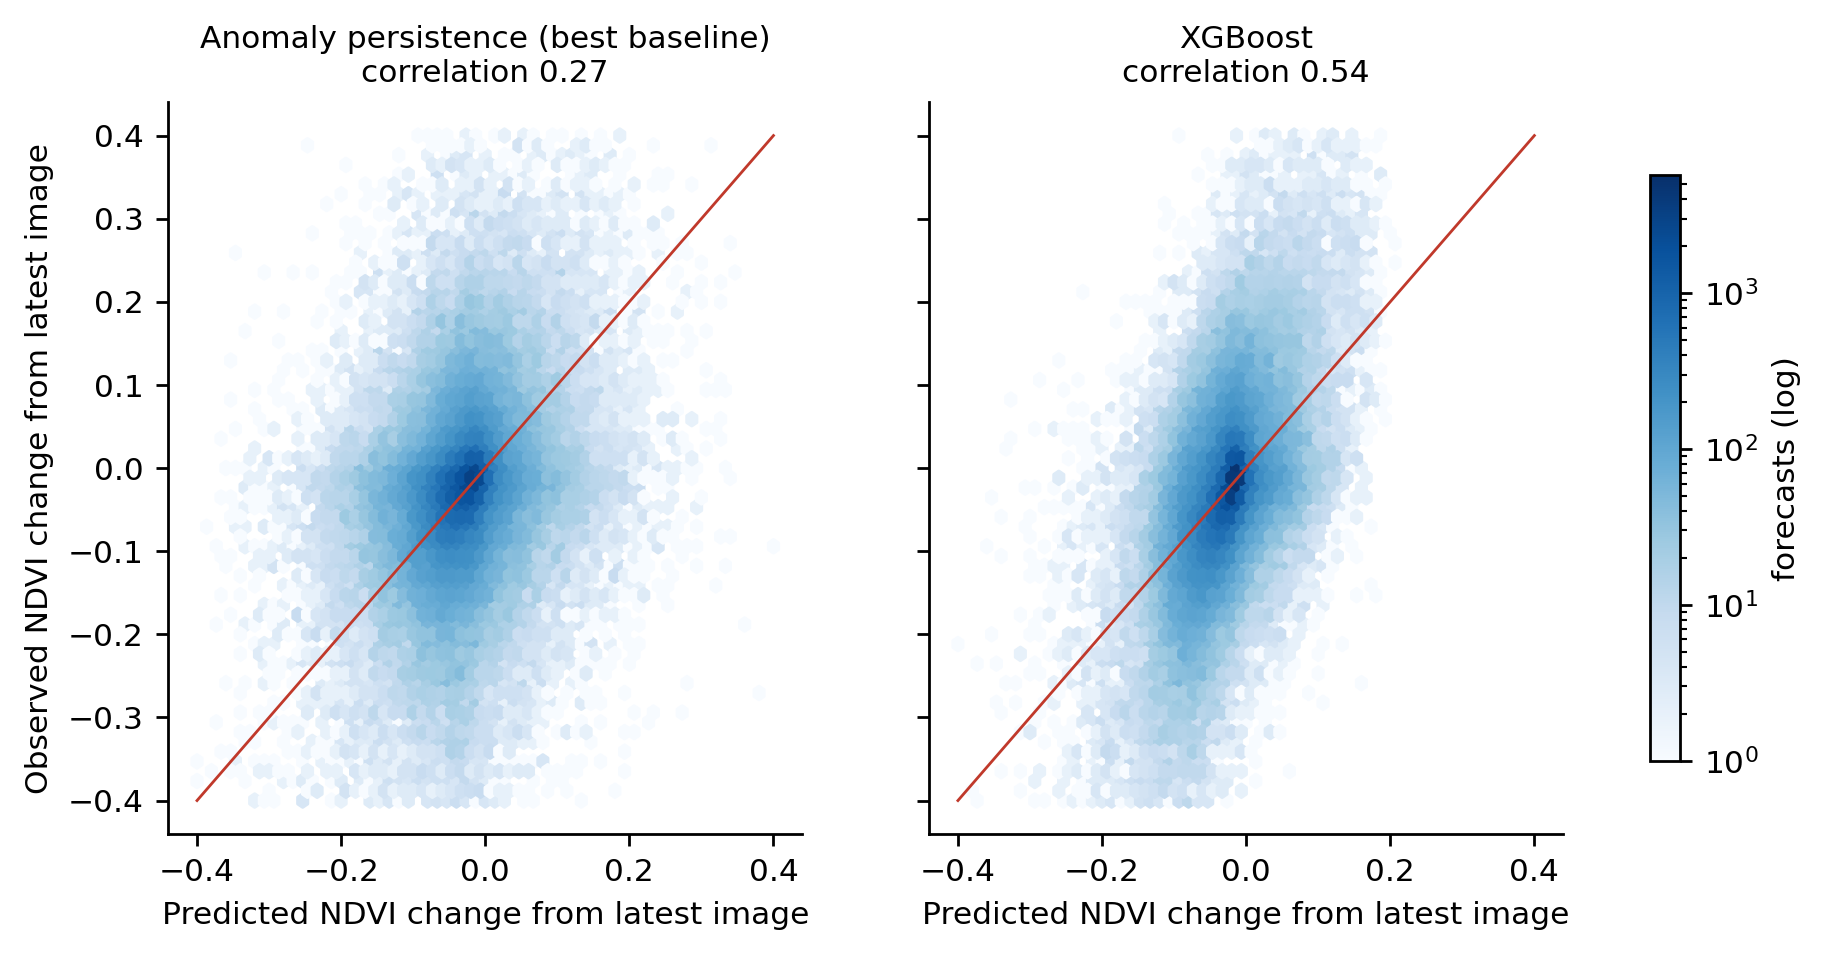
\includegraphics[width=0.85\textwidth]{figures/res_r_scatter.png}
\caption{Predicted vs observed 15-day NDVI change for the best baseline and XGBoost (all test forecasts; red line = perfect forecast).}
\label{fig:r_scatter}
\end{figure}

Figure~\ref{fig:r_examples} shows forecasts for four points drawn at random (fixed seed) from four mandals in the dry season 2023-24. XGBoost (blue) follows the observed curve more closely than persistence (grey), especially during green-up and gradual decline; sudden drops such as the mid-February fall at the Adoni point are only caught after they start.

\begin{figure}[H]
\centering
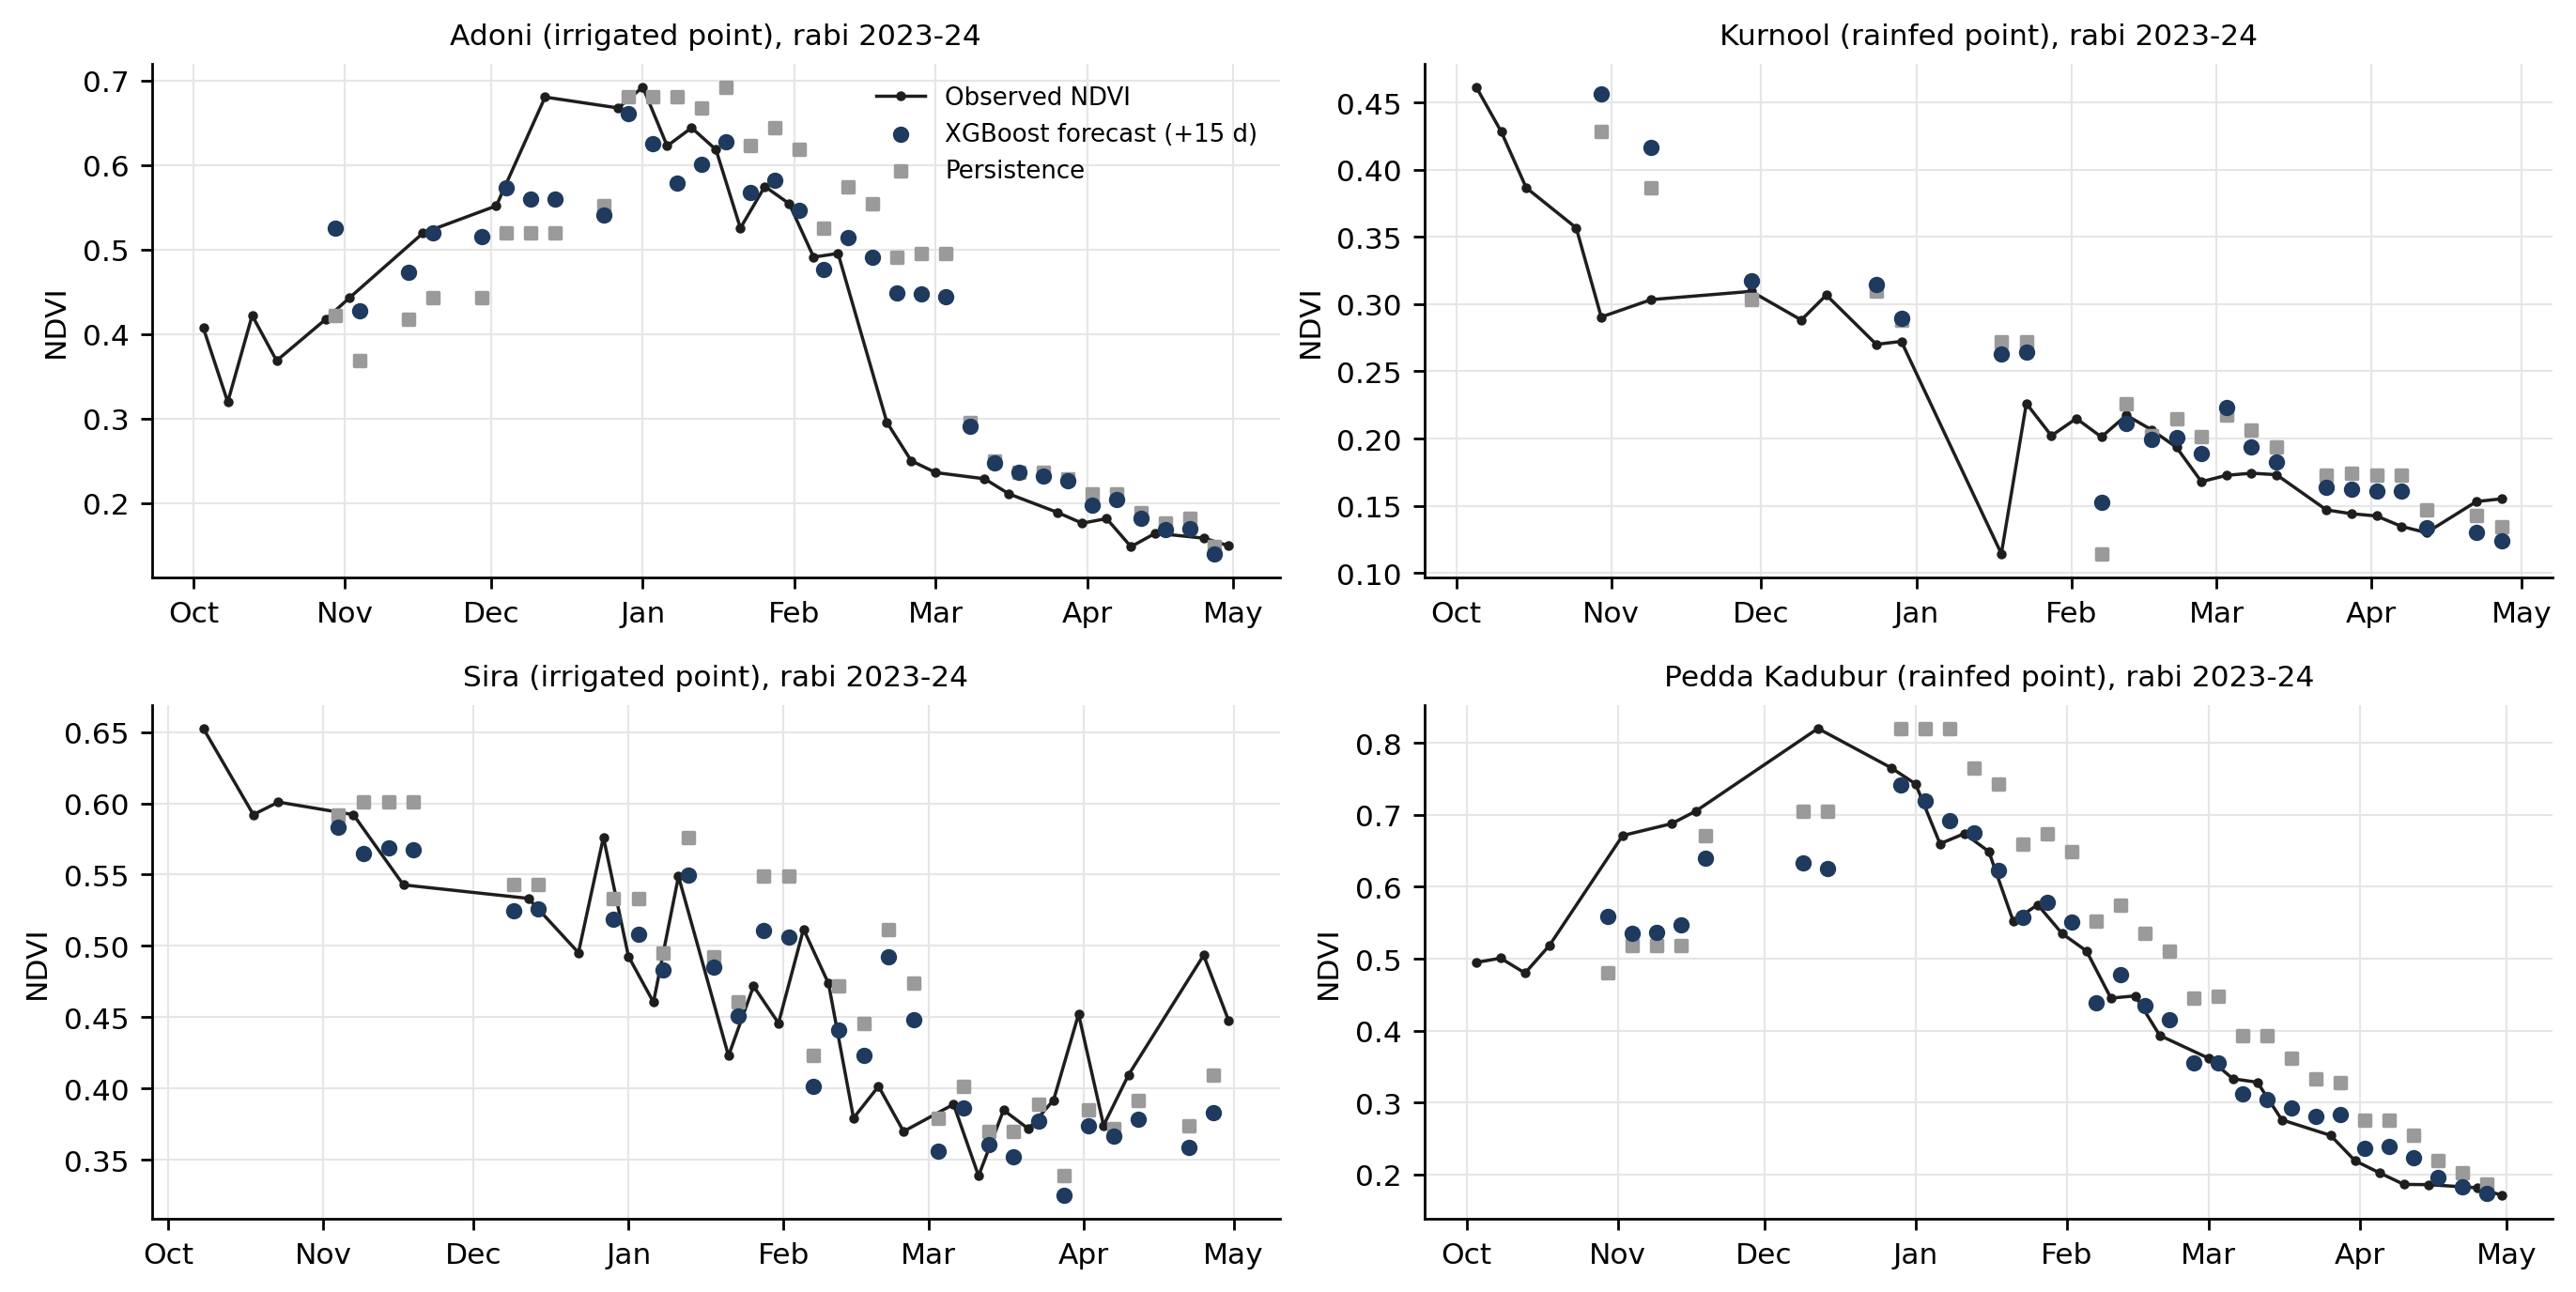
\includegraphics[width=\textwidth]{figures/res_r_examples.png}
\caption{Example forecasts at four random points, rabi 2023-24: observed NDVI (black), XGBoost forecast plotted at its target date (blue) and persistence (grey).}
\label{fig:r_examples}
\end{figure}

\subsubsection{Model versions and what the model uses}
Table~\ref{tab:r_versions} compares the model versions. The satellite-only model is as accurate as the main model: adding the tested weather features did not improve overall accuracy, and using weather with an unrealistic 1-day delay changes nothing either. The feature importance (Fig.~\ref{fig:r_importance}) confirms that the model relies mainly on recent satellite history (NDVI 15 and 30 days ago, season minimum), whether the point is irrigated, and the point's normal curve; the three weather variables among the top 12 (temperature, 90-day rain, water balance) together account for only about 11\,\% of the gain.

% --- table r_versions (generated by make_results.py)
\begin{table}[H]
\centering
\caption{Rabi forecast: pooled MAE of all model versions and baselines (test 2023-24 to 2025-26).}
\label{tab:r_versions}
\footnotesize
\begin{tabular}{@{}lcccccc@{}}
\toprule
\textbf{Population} & \textbf{XGBoost (main)} & \textbf{Satellite only} & \textbf{Weather 1 d late} & \textbf{Persistence} & \textbf{Climatology} & \textbf{Anomaly pers.} \\
\midrule
All eligible & 0.0511 & 0.0509 & 0.0510 & 0.0641 & 0.0909 & 0.0623 \\
Established & 0.0490 & 0.0487 & 0.0489 & 0.0618 & 0.0898 & 0.0597 \\
\bottomrule
\end{tabular}
\end{table}


\begin{figure}[H]
\centering
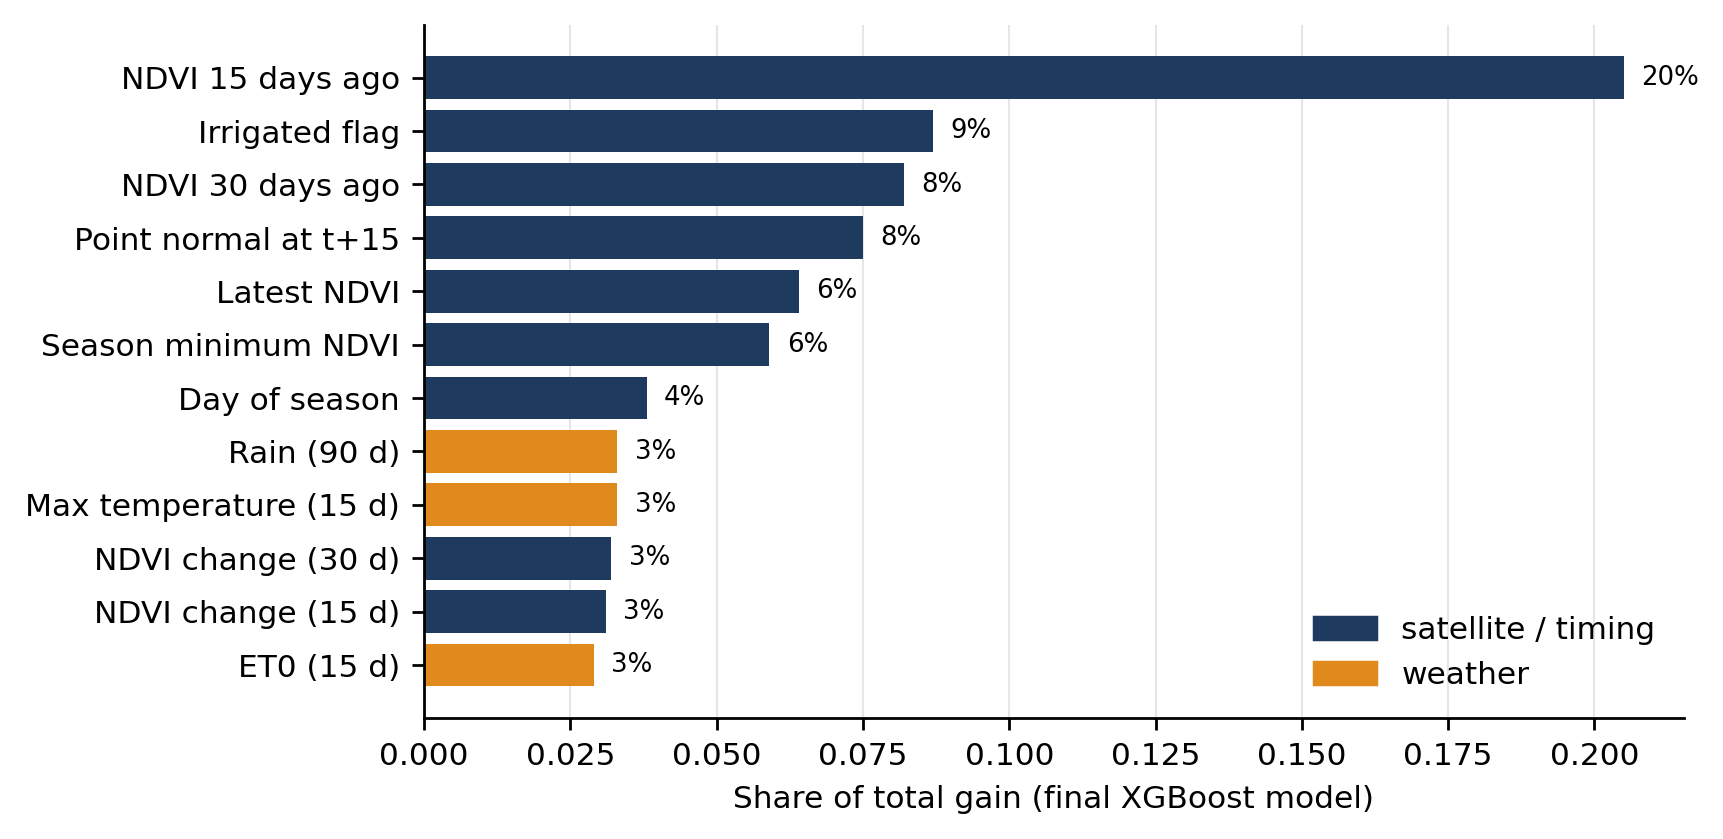
\includegraphics[width=0.7\textwidth]{figures/res_r_importance.png}
\caption{Feature importance of the final rabi XGBoost model (share of total gain; top 12 features).}
\label{fig:r_importance}
\end{figure}

\subsubsection{Warnings of declining greenness}
For established crops, a decline of at least 0.10 from the latest image to the forecast target (a span of 15--30 days, median 20) was flagged with 62\,\% precision and 24\,\% recall (AUC 0.83, against 0.65 for anomaly persistence): the warnings are selective and miss about three-quarters of declines, and a decline can be drought or harvest. These are historical evaluation results, not a prospective test or validation of drought detection.

% ============================================================================
\section{Module 3: UAV Drone Drought Segmentation}
% UAV-TODO: provisional text from the mid-review; replace with final method, dataset and results.

The UAV module processes ultra-high-resolution drone images (1.8--2.5\,mm ground sampling distance, DJI Mini~4 Pro flown at 10--12\,m above ground) over the flagged fields. A 9-channel input is built: RGB + ExG + ExGR + CIVE + GLI + NGRDI + HSV-V. A SegFormer-B2~\cite{segformer2021} model with an MiT-B2 encoder, a Spatially Adaptive Channel Attention (SACA) module and a Boundary-Aware Refinement (BAR) head segments 7 classes: Background, Soil, Healthy Crop, Cotton Ball, Green Weed, \textbf{Dry Weed} and \textbf{Drought}. Ground-truth masks are produced with a custom tile-based annotation tool (\texttt{TileAnnotator}) on $512 \times 512$ tiles. Training uses a class-imbalance-aware composite loss
\begin{equation}
\mathcal{L} = 1.0\,\mathcal{L}_{\text{Focal}}(\gamma=2) + 2.5\,\mathcal{L}_{\text{Dice}} + 1.0\,\mathcal{L}_{\text{Lov\'{a}sz}} + 0.2\,\mathcal{L}_{\text{BAR}}.
\end{equation}
To separate dry weeds from drought-stressed crops, an NGRDI constraint is applied, and the damaged area is computed as $A_d = N_{\text{drought}} \times \mathrm{GSD}^2$ (m$^2$).

\textbf{Dataset.} 2,254 drone images of 10 fields (November 2025 -- January 2026); 146 tiles annotated in 7 classes. \textit{Training and evaluation results will be added.}

\begin{figure}[H]
\centering
\resizebox{0.86\textwidth}{!}{%
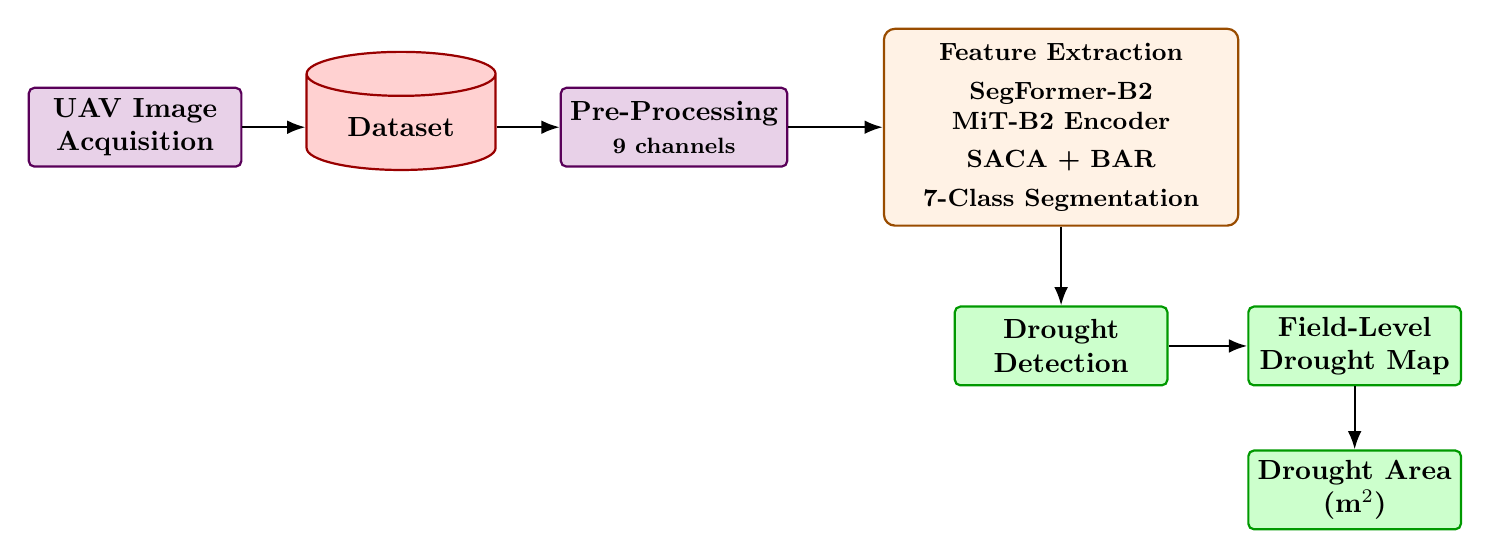
\begin{tikzpicture}[
    >=Latex,
    box/.style={rectangle, rounded corners=2pt, draw=violet!70!black, thick, fill=violet!18, align=center,
                minimum width=2.7cm, minimum height=1.0cm, font=\normalsize\bfseries},
    dataset/.style={cylinder, shape border rotate=90, aspect=0.35, draw=red!60!black, thick, fill=red!18,
                align=center, minimum width=2.4cm, minimum height=1.5cm, font=\normalsize\bfseries},
    model/.style={rectangle, rounded corners=4pt, draw=orange!60!black, thick, fill=orange!10, align=center,
                minimum width=4.5cm, minimum height=2.5cm, font=\small\bfseries},
    outbox/.style={rectangle, rounded corners=2pt, draw=green!60!black, thick, fill=green!20, align=center,
                minimum width=2.7cm, minimum height=1.0cm, font=\normalsize\bfseries},
    arrow/.style={->, >=Latex, thick}
]
\node[box] (uav) {UAV Image\\Acquisition};
\node[dataset, right=8mm of uav] (dataset) {Dataset};
\node[box, right=8mm of dataset] (preprocess) {Pre-Processing\\\footnotesize 9 channels};
\node[model, right=12mm of preprocess] (model) {Feature Extraction\\[1mm] SegFormer-B2\\ MiT-B2 Encoder\\[1mm] SACA + BAR\\[1mm] 7-Class Segmentation};
\node[outbox, below=10mm of model] (drought) {Drought\\Detection};
\node[outbox, right=10mm of drought] (field) {Field-Level\\Drought Map};
\node[outbox, below=8mm of field] (area) {Drought Area\\(m$^2$)};
\draw[arrow] (uav.east) -- (dataset.west);
\draw[arrow] (dataset.east) -- (preprocess.west);
\draw[arrow] (preprocess.east) -- (model.west);
\draw[arrow] (model.south) -- (drought.north);
\draw[arrow] (drought.east) -- (field.west);
\draw[arrow] (field.south) -- (area.north);
\end{tikzpicture}%
}
\caption{UAV module architecture (provisional).}
\label{fig:uav_arch}
\end{figure}

% ============================================================================
\section{Discussion}
\begin{itemize}
\item \textbf{Physics and machine learning.} The physical water-balance ensemble is a strong baseline; machine learning adds significant skill mainly at 15 days, and nothing is skilful at 30 days. Reporting this honestly is a strength of the work.
\item \textbf{Weather as a ``where to look'' signal.} Rainfed crop stress follows meteorological drought by about 10 days, so a weather alarm is a useful trigger for satellite checking.
\item \textbf{Weather adds little to crop forecasts.} In both kharif (15--30 days) and rabi (15 days), crop condition is set mostly by water already lost; satellite history carries most of the forecast skill.
\item \textbf{Declarations are administrative decisions.} Agreement is strong for severe kharif droughts and weak for moderate and rabi cases; declarations are therefore used only as a comparison, never as a training target.
\item \textbf{Rabi needs its own design.} Stored soil water, irrigation and terminal drought make rabi different; forecasting greenness avoids training on a handful of declarations.
\end{itemize}

\textbf{Novelty.}
\begin{table}[H]
\centering
\caption{Comparison with common practice.}
\label{tab:novelty}
\footnotesize
\begin{tabularx}{\textwidth}{@{}p{2.4cm}p{4.2cm}Y@{}}
\toprule
\textbf{Aspect} & \textbf{Common practice} & \textbf{This work} \\
\midrule
Baselines & Other ML models & Persistence, Markov, climatology and a physical water-balance ensemble \\
Calibration & Full record & SPEI frozen on 1979--2011; SVI normals on 2019--2023 with the scored year removed \\
Leakage & Rarely tested & 42 automated tests, independent reviews, purged splits \\
Fields & Hand-picked or district averages & Automatic farmland mapping; 240 random fields and 1,350 random points \\
Validation & Index vs index & Four seasons of government orders, live replay with data delays, UAV fields \\
Rabi & Post-hoc coarse indices & 10\,m greenness forecast with rules registered before training \\
\bottomrule
\end{tabularx}
\end{table}

% ============================================================================
\section{Limitations}
\begin{itemize}
\item Short satellite record: normals rest on five years, and there are few drought events, so agreement figures are case evidence.
\item Monsoon clouds often leave fewer than 5 clear fields in August--September, delaying confirmation.
\item SVI classes are index categories, not measured damage; irrigation is inferred from dry-season greenness.
\item Spatial mismatch between mandals, 3\,km areas and fields (e.g.\ 70\,\% of Peddakadubur fields lie in Pedda Kadubur although the centre is in Adoni).
\item AgERA5 is about a week late, so a 7-day weather forecast gives little real warning; 15 days gives about a week.
\item Rabi: evaluated on seasons known during design; it forecasts NDVI, not drought; points are sampled pixels, not verified fields; only five weather cells and three test seasons.
\item UAV flights were post-harvest; agreement with satellite verdicts is weak at single dates (3 of 10 fields clear, 2 mixed).
\end{itemize}

% ============================================================================
\section{Conclusion and Future Work}
This project built and evaluated a weather-to-satellite drought early-warning chain for Rayalaseema with strict leakage control and honest baselines. The hybrid weather model forecasts the SPEI-30 class with \mf{} 0.819 at 7 days and 0.651 at 15 days; rainfed crops respond about 10 days after meteorological drought; and the chain confirmed all 9 severe kharif drought site-seasons of 2023--2026, five before the government order, with one false alarm in eleven undeclared site-seasons. For rabi, a 15-day NDVI forecast had about 18\,\% lower error than the best simple baseline on three held-out seasons.

\textbf{Future work:} (i) a prospective test on rabi 2026-27 and kharif 2027 with the frozen rules; (ii) independent agricultural-drought validation with yield statistics and field surveys; (iii) a soil-water balance with soil-specific storage for rabi; (iv) completing UAV training and linking satellite-flagged fields to drone damage maps in m$^2$.

\textbf{Code and data:} github.com/ARYAN3012-G/weather\_time\_series $\cdot$ github.com/ARYAN3012-G/Sentinel2-Drought-Confirmation $\cdot$ github.com/ARYAN3012-G/Rabi-Drought-Monitoring-

% ============================================================================
\section{References}
\begingroup
\small
\setlength{\parskip}{0pt}
\renewcommand{\section}[2]{}
\begin{thebibliography}{40}
\setlength{\itemsep}{0pt}
\setlength{\parsep}{0pt}

\bibitem{manual2016} Government of India, \textit{Manual for Drought Management}, Ministry of Agriculture and Farmers Welfare, New Delhi, 2016 (updated 2020).

\bibitem{bhardwaj2021} K.~Bhardwaj and V.~Mishra, ``Drought detection and declaration in India,'' \textit{Water Security}, vol.~14, p.~100104, 2021.

\bibitem{vicente2010} S.~M.~Vicente-Serrano, S.~Beguer\'{i}a, and J.~I.~L\'{o}pez-Moreno, ``A multiscalar drought index sensitive to global warming: the Standardized Precipitation Evapotranspiration Index,'' \textit{J.\ Climate}, vol.~23, no.~7, pp.~1696--1718, 2010.

\bibitem{belayneh2014} A.~Belayneh, J.~Adamowski, B.~Khalil, and B.~Ozga-Zielinski, ``Long-term SPI drought forecasting in the Awash River Basin in Ethiopia using wavelet neural network and wavelet support vector regression models,'' \textit{J.\ Hydrology}, vol.~508, pp.~418--429, 2014.

\bibitem{dikshit2021} A.~Dikshit, B.~Pradhan, and A.~Huete, ``An improved SPEI drought forecasting approach using the long short-term memory neural network,'' \textit{J.\ Environ.\ Manage.}, vol.~283, p.~111979, 2021.

\bibitem{prodhan2022} F.~A.~Prodhan, J.~Zhang, S.~S.~Hasan, T.~P.~Pangali Sharma, and H.~P.~Mohana, ``A review of machine learning methods for drought hazard monitoring and forecasting: current research trends, challenges, and future research directions,'' \textit{Environ.\ Model.\ Softw.}, vol.~149, 2022.

\bibitem{marusov2024} A.~Marusov, V.~Grabar, Y.~Maximov \textit{et al.}, ``Long-term drought prediction using deep neural networks based on geospatial weather data,'' \textit{Environ.\ Model.\ Softw.}, vol.~179, 2024; arXiv:2309.06212.

\bibitem{allen1998} R.~G.~Allen, L.~S.~Pereira, D.~Raes, and M.~Smith, \textit{Crop Evapotranspiration: Guidelines for Computing Crop Water Requirements}, FAO Irrigation and Drainage Paper 56, Rome, 1998.

\bibitem{agera5} H.~Boogaard \textit{et al.}, ``Agrometeorological indicators from 1979 to present derived from reanalysis (AgERA5),'' Copernicus Climate Change Service (C3S) Climate Data Store.

\bibitem{chen2016} T.~Chen and C.~Guestrin, ``XGBoost: a scalable tree boosting system,'' in \textit{Proc.\ 22nd ACM SIGKDD}, pp.~785--794, 2016.

\bibitem{breiman2001} L.~Breiman, ``Random forests,'' \textit{Machine Learning}, vol.~45, no.~1, pp.~5--32, 2001.

\bibitem{kogan1995} F.~N.~Kogan, ``Application of vegetation index and brightness temperature for drought detection,'' \textit{Adv.\ Space Res.}, vol.~15, no.~11, pp.~91--100, 1995.

\bibitem{peters2002} A.~J.~Peters, E.~A.~Walter-Shea, L.~Ji, A.~Vi\~{n}a, M.~Hayes, and M.~D.~Svoboda, ``Drought monitoring with NDVI-based Standardized Vegetation Index,'' \textit{Photogramm.\ Eng.\ Remote Sens.}, vol.~68, no.~1, pp.~71--75, 2002.

\bibitem{rhee2010} J.~Rhee, J.~Im, and G.~J.~Carbone, ``Monitoring agricultural drought for arid and humid regions using multi-sensor remote sensing data,'' \textit{Remote Sens.\ Environ.}, vol.~114, no.~12, pp.~2875--2887, 2010.

\bibitem{park2016} S.~Park, J.~Im, E.~Jang, and J.~Rhee, ``Drought assessment and monitoring through blending of multi-sensor indices using machine learning approaches for different climate regions,'' \textit{Agric.\ Forest Meteorol.}, vol.~216, pp.~157--169, 2016.

\bibitem{padhee2014} S.~K.~Padhee, B.~R.~Nikam, S.~P.~Aggarwal, and V.~Garg, ``Integrating effective drought index (EDI) and remote sensing derived parameters for agricultural drought assessment and prediction in Bundelkhand region of India,'' \textit{ISPRS Arch.}, vol.~XL-8, pp.~89--100, 2014.

\bibitem{nikam2020} B.~R.~Nikam \textit{et al.}, ``Assessment of early season agricultural drought using remote sensing,'' \textit{ISPRS Arch.}, vol.~XLIII-B3-2020, pp.~1691--1695, 2020.

\bibitem{asoka2015} A.~Asoka and V.~Mishra, ``Prediction of vegetation anomalies to improve food security and water management in India,'' \textit{Geophys.\ Res.\ Lett.}, vol.~42, no.~13, pp.~5290--5298, 2015.

\bibitem{descals2025} A.~Descals, K.~Torres, A.~Verger, and J.~Pe\~{n}uelas, ``Evaluating Sentinel-2 for monitoring drought-induced crop failure in winter cereals,'' \textit{Remote Sens.}, vol.~17, no.~2, p.~340, 2025.

\bibitem{sharma2025} S.~S.~Sharma, J.~Mukherjee, and F.~Dell'Acqua, ``Leveraging Sentinel-2 data and machine learning for drought detection in India: the process of ground truth construction and a case study,'' \textit{Remote Sens.}, vol.~17, no.~18, p.~3159, 2025.

\bibitem{pang2017} J.~Pang \textit{et al.}, ``Pattern of water use and seed yield under terminal drought in chickpea genotypes,'' \textit{Front.\ Plant Sci.}, vol.~8, p.~1375, 2017.

\bibitem{gorelick2017} N.~Gorelick, M.~Hancher, M.~Dixon, S.~Ilyushchenko, D.~Thau, and R.~Moore, ``Google Earth Engine: planetary-scale geospatial analysis for everyone,'' \textit{Remote Sens.\ Environ.}, vol.~202, pp.~18--27, 2017.

\bibitem{drusch2012} M.~Drusch \textit{et al.}, ``Sentinel-2: ESA's optical high-resolution mission for GMES operational services,'' \textit{Remote Sens.\ Environ.}, vol.~120, pp.~25--36, 2012.

\bibitem{pasquarella2023} V.~J.~Pasquarella, C.~F.~Brown, W.~Czerwinski, and W.~J.~Rucklidge, ``Comprehensive quality assessment of optical satellite imagery using weakly supervised video learning,'' in \textit{Proc.\ CVPR Workshops}, 2023.

\bibitem{achanta2017} R.~Achanta and S.~S\"{u}sstrunk, ``Superpixels and polygons using simple non-iterative clustering,'' in \textit{Proc.\ CVPR}, 2017.

\bibitem{zanaga2022} D.~Zanaga \textit{et al.}, ``ESA WorldCover 10\,m v100 / v200,'' 2021, 2022.

\bibitem{brown2022} C.~F.~Brown \textit{et al.}, ``Dynamic World, near real-time global 10\,m land use land cover mapping,'' \textit{Scientific Data}, vol.~9, p.~251, 2022.

\bibitem{shahi2023} T.~B.~Shahi, C.-Y.~Xu, A.~Neupane, G.~Fresser, and W.~Guo, ``Classification of water stress in cotton using convolutional neural networks from UAV images,'' \textit{Remote Sens.}, vol.~15, no.~1, p.~35, 2023.

\bibitem{dang2023} F.~Dang, D.~Chen, Y.~Lu, and Z.~Li, ``Deep learning-based weed detection using UAV images: a comparative study,'' \textit{Drones}, vol.~7, no.~1, p.~2, 2023.

\bibitem{segformer2021} E.~Xie, W.~Wang, Z.~Yu, A.~Anandkumar, J.~M.~Alvarez, and P.~Luo, ``SegFormer: simple and efficient design for semantic segmentation with Transformers,'' in \textit{Proc.\ NeurIPS}, 2021.

\end{thebibliography}
\endgroup

\vspace{6pt}
\noindent\rule{0.38\textwidth}{0.4pt}\hfill\rule{0.28\textwidth}{0.4pt}\\[2pt]
\noindent\textbf{Guide's Signature}\hfill\textbf{Date}

\end{document}
